\documentclass[a4paper,11pt]{report}
\usepackage[]{amsmath}
\usepackage[]{physics} % \bra, \ket etc
\usepackage{graphicx} %Pour les figures je crois
\usepackage{hyperref}
\usepackage[
    backend=biber, 
    natbib=true,
    style=numeric-comp,
    sorting=none, %Pour faire apparaitre les refs dans l'ordre
    hyperref=true
]{biblatex} %Imports biblatex package
\addbibresource{Bib_ch4.bib} %Import the bibliography file

\usepackage{amssymb} %quelques symboles dont gtrsim /lesssim
\usepackage{subcaption} % package pour faire des subfigures
\usepackage{multirow} % package pour multirow/multicolumn
\usepackage{booktabs} % package pour top/mid/bottom rule
\usepackage{tcolorbox} % toujours plus de boites
\usepackage{xcolor} % Pour avoir des couleurs dans les équations

\DeclareUnicodeCharacter{0308}{HERE!HERE!} % je vais pas m'énerver, mais un peu quand meme
\title{}
\begin{document}
\chapter{NV-NV CR under transverse or low fields: application to magnetometry}

In the last chapter we saw how dense ensemble of NV centers have an intrinsic depolarization mechanism mediated by the NV-NV dipole interaction. In this chapter we will see how this feature can be exploited to perform magnetometry. 

Using NV-NV CR for magnetometry in non-zero magnetic field has already been proposed \citep{akhmedzhanov2017microwave, akhmedzhanov2019magnetometry}. We will focus here on the low to zero magnetic field region, which presents practical advantages as the relative orientation of the diamond with the magnetic field does not need to be controlled, but theoretical complications due to the more complex physics of the NV centers under low magnetic field.

This chapter is constructed as follows: We will first describe the physics of NV centers under low or transverse magnetic field (the physics is similar in both cases), we will then show both theoretically and experimentally that the NV-NV CR is modified for low and transverse magnetic field. We will identify different mechanisms by which the relaxation is modified and we will try to quantify their relative importance.

We will then focus on the low field depolarization magnetometry (LFDM) protocol which exploits the previously studied NV-NV CR at low magnetic field. We will start by giving a short overview of NV ensemble magnetometry before characterizing the LFDM protocol and comparing it to other magnetometry protocols. Finally we will give some perspectives on how to improve LFDM and on potential applications.

The results presented in this chapter are based in large part on the article \citep{pellet2022spin}.

\section{NV spin Hamiltonian under low and transverse fields}

Before looking at the NV-NV CR in the low or transverse field regime, we first need to consider how the general NV physics is modified under those regimes, and in particular we need to look at the modifications of the spin Hamiltonian and the change in the eigenstates compared to the high magnetic field regime.

\subsection{NV spin Hamiltonian in zero external magnetic field}
\begin{figure}[h]
\centering
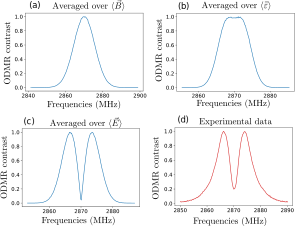
\includegraphics[width=\textwidth]{Figures/ESR_simus}
\caption{Simulations of inhomogeneous zero field ODMR when sampling various parameters. a) Simulation when sampling each components of the magnetic field over a Gaussian of deviation $\sigma=2\ \rm G$. b) Simulation when sampling each components of the strain tensor $\bar{\bar{\varepsilon}}$ over a Gaussian of deviation $\sigma=2\cdot 10^{-4}$. c) Simulation when sampling each components of the electric field over a Gaussian of deviation $\sigma=2\cdot 10^{5}\ \rm{V/cm}$. d) Experimental ODMR spectrum in zero external field taken on sample ADM-150-2}
\label{simus ESR}
\end{figure}

In the absence of external magnetic field, we have to take into account other elements which would otherwise be of second order in the spin Hamiltonian. These elements are: the random local magnetic fields caused by paramagnetic impurities, the local electric field caused by charged impurities, and the crystal strain \citep{doherty2012theory, udvarhelyi2018spin, mittiga2018imaging}. The hyperfine splitting due to nearby nuclei will be considered separately, although to a large extent it behaves like a local magnetic field.

Due to the large zero field splitting $D=2870\ \rm MHz$ between the $\ket{0}$ and $\ket{\pm 1}$ states, we will consider the $\ket{0}$ state to always be an eigenstate of the spin Hamiltonian under zero external field (which is equivalent to say that we neglect the terms in $\ket{0}\bra{\pm 1}$ in the spin Hamiltonian). The problem is then reduced to the $\{ \ket{-1}, \ket{+1} \}$ subsystem.

The NV$^-$spin Hamiltonian in the $\{ \ket{-1}, \ket{+1} \}$ basis can be written as \citep{udvarhelyi2018spin}:
\begin{equation}
\mathcal{H}=\begin{pmatrix}
D-\gamma_e B_\parallel + f_\parallel(\mathbf{E}) + g_\parallel(\bar{\bar{\varepsilon}}) & f_\perp(\mathbf{E}) + g_\perp(\bar{\bar{\varepsilon}})\\
f^*_\perp(\mathbf{E}) + g^*_\perp(\bar{\bar{\varepsilon}})&D+\gamma_e B_\parallel + f_\parallel(\mathbf{E}) + g_\parallel(\bar{\bar{\varepsilon}})
\end{pmatrix},
\label{Hamiltonien pm1}
\end{equation}
where $B_\parallel$ is the component of the magnetic field along the NV axis, and $f_\parallel, f_\perp, g_\perp$, and $g_\parallel$ are functions of the electric field $\mathbf{E}$ and the strain tensor $\bar{\bar{\varepsilon}}$, whose expressions are:

\begin{align}
f_\parallel(\mathbf{E})&=d_\parallel E_z, \\
f_\perp(\mathbf{E})&=d_\perp ( E_x + i E_y), \\
g_\parallel(\bar{\bar{\varepsilon}})&= h_{41}(\varepsilon_{xx}+\varepsilon_{yy})+h_{43} \varepsilon_{zz}, \\
g_\perp(\bar{\bar{\varepsilon}}) &= \frac{1}{2} \left[ h_{16}(\varepsilon_{zx}+i \varepsilon_{zy}) + h_{15}\left(\frac{\varepsilon_{yy}-\varepsilon_{xx}}{2}+i\varepsilon_{xy}\right) \right],
\end{align}
where $d_\parallel=0.35 \ \rm{Hz\, cm/V}$ and $d_\perp=17\ \rm{Hz\, cm/V}$ have been measured experimentally \citep{van1990electric}, and $h_{43}=2300\ \rm{MHz}$, $h_{41}=-6420\ \rm{MHz}$, $h_{15}=5700\ \rm{MHz}$ and $h_{16}=19660\ \rm{MHz}$ were computed through DFT \citep{udvarhelyi2018spin} and show reasonable agreement with experiments \citep{barson2017nanomechanical}.

Importantly, as pointed in \citep{mittiga2018imaging} we notice that both the electric field and the strain have a \textit{shifting} component ($f_\parallel$ and $g_\parallel$) which shifts equally both eigenstates of the Hamiltonian, and a \textit{splitting} component ($f_\perp$ and $g_\perp$) which splits in energy the two eigenstates. 

The main difference between the electric field and the strain is in the numerical prefactors of these components: for the electric field, the splitting parameter $d_\perp$ is $\sim 50$ times higher than the shifting parameter $d_\parallel$, which will result on average to a strong energy split without much shifting. For the strain however, the splitting parameters $h_{15}$ and $h_{16}$ are only $\sim 3$ times higher than the shifting parameters $h_{43}$ and $h_{41}$. The shift in energy will therefore tend to blur the energy split when averaging over a large number of spins.

Fig. \ref{simus ESR} shows a simulation of how each parameters of the spin Hamiltonian - local magnetic field, local electric field and strain - affects the zero external field ODMR profile. To do these simulations, I sampled each parameters separately $10^6$ times and plotted the histogram of the two eigenvalues of the Hamiltonian written in eq. \ref{Hamiltonien pm1}. Fig. \ref{simus ESR}-d) shows an experimental zero field ODMR spectrum, typical of what we observe with dense NV ensembles. 

Experimentally, almost all our samples show the characteristic two bumps in zero external field ODMR. Given the simulation results, the only parameter that can give rise to this shape is the local electric field. 

We should note that another potential explanation for the splitting of the $\ket{\pm 1}$ states could be the presence of a residual magnetic field, not randomly distributed among all the spins but homogeneous on the whole sample. In particular, we do not shield for the earth magnetic field in our experiment. The splitting caused by the earth magnetic field however has a value $\gamma B_{\rm earth} \approx 1\ \rm MHz$, which is $\sim 4$ times weaker than the splitting we typically observe. 

We will therefore consider that the low external magnetic field spin Hamiltonian of our samples is dominated by the local electric field, and more specifically by the transverse electric field $E_\perp\equiv E_x + i E_y$ given the ratio between $d_\perp$ and $d_\parallel$.

We will then adopt the following simplified Hamiltonian for the zero external field regime:
\begin{equation}
\mathcal{H}=\begin{pmatrix}
D&0&d_\perp E_\perp^* \\
0&0&0 \\
d_\perp E_\perp &0&D
\end{pmatrix},
\end{equation}
whose eigenvectors are $\ket{0}$ and$\ket{\pm}$ of eigenvalues 0 and $D\pm d_\perp \abs{E_\perp}$, where $\ket{\pm}$ are defined as:
\begin{equation}
\ket{\pm}=\frac{\ket{+1}\pm e^{-i\phi_E}\ket{-1}}{\sqrt{2}},
\end{equation}
where $\tan(\phi_E)=E_y/E_x$.

\subsection{NV spin Hamiltonian under purely transverse magnetic field}
\label{sec B transverse}
%\begin{figure}[h]
%\centering
%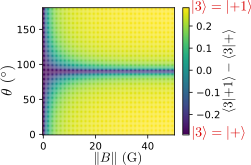
\includegraphics[width=0.7\textwidth]{Figures/map_etats_propres}
%\caption{Closeness of the Hamiltonian most excited state $\ket{3}$ with either $\ket{+1}$ or $\ket{+}$ as a function of the external magnetic field amplitude and angle $\theta$ with respect to the NV axis.}
%\label{map champ transverse}
%\end{figure}

We now turn to the case of purely transverse magnetic field with respect to the NV axis, i.e. $\mathbf{B}=B_x \hat{e}_x + B_y \hat e_y$, and more specifically to the regime where $d_\perp E_\perp < \frac{(\gamma_e B_\perp)^2}{D} << D$. In practice, this generally corresponds to $20\ \rm G \lesssim B_\perp \lesssim 200\ \rm G$.

In this regime, the NV Hamiltonian eigenstates are similar to the case where it is dominated by the transverse electric field and can be written $\approx \ket{0}, \ket{-}, \ket{+}$\citep{qiu2021nuclear, qiu2022nanoscale}, of respective eigenvalues $\approx -\frac{(\gamma_e B_\perp)^2}{D},D,D+\frac{(\gamma_e B_\perp)^2}{D}$,  where:
\begin{equation}
\ket{\pm}=\frac{\ket{+1}\pm e^{-2i\phi_B}\ket{-1}}{\sqrt{2}},
\end{equation}
and $\tan(\phi_B)=B_y/B_x$.

For the case where $d_\perp E_\perp \sim \frac{(\gamma_e B_\perp)^2}{D}$ and $\phi_E \neq 2\phi_B$, the eigenstates of the Hamiltonian are still of the form $\ket{0},\ket{\pm}$ with a relative angle $\phi$ in between $\phi_E$ and $2\phi_B$.

In conclusion, whenever the spin Hamiltonian is dominated by a transverse field, either electric or magnetic, we can consider that the eigenstates of the spin Hamiltonian to be $\ket{0}, \ket{-}$ and $\ket{+}$, whereas when the Hamiltonian is dominated by the longitudinal magnetic field, its eigenstates are $\ket{0}, \ket{-1}$ and $\ket{+1}$.

\subsection{Hyperfine coupling and inhomogeneous broadening}
\label{sec modif T2*}
\begin{figure}[h]
\centering
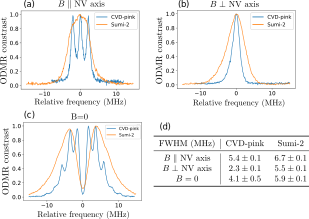
\includegraphics[width=\textwidth]{Figures/Comparaison_ESR_T2}
\caption{ODMR lineshapes for longitudinal, transverse and low magnetic fields on samples CVD-pink and Sumi-2. a) ODMR spectrum of a single class of NV centers for a longitudinal magnetic field ($B_\parallel \sim 100\ \rm G$). The microwave frequency is given with respect to the ODMR line central frequency. b) ODMR spectrum of a single class for a purely transverse magnetic field ($B_\perp \sim 100\ \rm G$). c) ODMR of all 4 classes for 0 external magnetic field. d) Table reporting the full width at half maximum of each ODMR line.}
\label{ESR for T2*}
\end{figure}

We will now look at the modification in the ODMR linewidths caused by the different magnetic field regimes. These change are relevant to our study of NV-NV CR due to the relation between the dipole-induced relaxation rate and $T_2^*$ detailed in sec. [REF].

A consequence of the change in the Hamiltonian eigenstates from the $\{ \ket{0}, \ket{\pm 1} \}$ to the $\{ \ket{0}, \ket{\pm} \}$ basis is that the Hamiltonian eigenvalues are sensitive to different part of the environment. In the $\{ \ket{0}, \ket{\pm 1} \}$, the eigen energies are linearly sensitive to (longitudinal) magnetic field, and only sensitive to electric fields at the second order, and vice versa for the $\{ \ket{0}, \ket{\pm} \}$ basis.

These different sensitivities affect both the inhomogeneous broadening, due to the local electric and magnetic noise, and the hyper-fine coupling to the various surrounding nuclei. These effects can drastically modify the ODMR lineshape in zero external magnetic field \citep{jamonneau2016competition} or purely transverse magnetic field \citep{qiu2021nuclear,qiu2022nanoscale}.

We will only consider here the hyper-fine splitting caused by the $^{14}$N nuclei of the nitrogen atom forming the NV center. $^{14}$N represents 99.6 \% of natural abundance nitrogen atoms, and it has an $I=1$ nuclear spin. The full $3\times 3$ Hamiltonian of the NV center in these conditions can be written:
\begin{equation}
\mathcal{H}=\mathcal{H}_e + \mathcal{H}_n + \mathbf{S} \bar{\bar{A}} \mathbf{I},
\end{equation}

where $\mathbf{S}$ is the electronic spin operator, $\mathbf{I}$ the nuclear spin operator, $\mathcal{H}_e$ the previously described electronic spin Hamiltonian, $\mathcal{H}_n$ the nuclear spin Hamiltonian and $\bar{\bar{A}}$ the hyper fine tensor. $\mathcal{H}_n$ and $\bar{\bar{A}}$ can be written:

\begin{equation}
\mathcal{H}_n = \gamma_N \mathbf{I} \cdot \mathbf{B} + Q I_z^2,
\end{equation}

and
\begin{equation}
\bar{\bar{A}} = \begin{pmatrix}
A_{xx} & 0 & 0 \\
0 & A_{yy} & 0 \\
0 & 0 & A_{zz}
\end{pmatrix},
\end{equation}


where $\gamma_N=0.308\ \rm kHz/G$, $Q=-4.945\ \rm MHz$, $A_{zz}=-2.162\ \rm MHz$ and $A_{xx}=A_{yy}=-2.62\ \rm MHz$ \citep{smeltzer2009robust}.

Fig. \ref{ESR for T2*} shows ODMR spectra for two samples, CVD-pink and Sumi-2, in three magnetic configuration: for a strong longitudinal magnetic field, where the NV eigenbasis is $\{ \ket{0}, \ket{\pm 1} \}$, and for a strong transverse magnetic field or no magnetic field, where the NV eigenbasis is $\{ \ket{0}, \ket{\pm} \}$. 

While both samples are relatively equivalent in term of NV concentration ([NV]=$3 \sim 5$ ppm), sample Sumi-2 contains significantly more impurities besides NV centers, most likely P1 centers. These impurities cause both magnetic (because of paramagnetic impurities) and electric (because of charged impurities) field noise.

Fig. \ref{ESR for T2*}-a) allows us to evaluate the magnetic field noise in both samples, since the $\ket{\pm 1}$ states are not sensitive to weak electric fields. We indeed find that the Sumi-2 sample has much more magnetic noise, to the point where the hyper-fine structure is no longer resolved. The total width of the line however is mostly dominated by the hyper-fine splitting, which result in a similar total linewidth in both cases

We should note that the usual practice in magnetometry is to consider the linewidth only of the three hyper-fine lines when they are resolved. This is because magnetometry protocol usually relies on a microwave field with a very well defined frequency, which can effectively select only one of the lines. In our case however, we have to consider the spectral overlap between NV centers and fluctuators, which have an additional broadening of $2\gamma_f \approx 6\ \rm MHz$ [REF] that completely obscures the hyper-fine structure. We therefore have to consider the full linewidth, even when the hyper-fine structure is resolved.

Fig. \ref{ESR for T2*}-b) allows us to evaluate the electric field noise in both samples, since the $\ket{\pm}$ states are not sensitive to weak magnetic fields. Similarly, the hyper-fine structure is hidden in this configuration since all three hyper-fine levels are nearly-degenerate, provided that $\frac{(\gamma_e B_\perp)^2}{D} > A_{xx},A_{zz},Q$ which is typically the case for $B_\perp > 40\ \rm G$. We can note that the electric field noise is significantly stronger in sample Sumi-2, which leads to an ODMR linewidth more than twice as big.

Finally, \ref{ESR for T2*}-c) shows the linewidth of both samples for zero external magnetic field. For sample Sumi-2, the profile and linewidth is similar to the case of the purely transverse magnetic field, which is consistent with the fact that the electric field noise is stronger than the residual magnetic fields (earth magnetic field and hyper-fine interaction). For sample CVD-pink however, the electric field noise is smaller than the hyper-fine interaction, meaning that only the $\ket{m_s=-1,m_I=+1}$ and $\ket{m_s=+1,m_I=-1}$ states (the ones closest to the central dip) will be dominated by the electronic noise, and be in the electronic states $\ket{m_e=\pm}$. The $\ket{m_I=\pm 1}$ states are dominated by the hyper-fine field and are in the electronic $\ket{m_e=\pm 1}$ basis.

The table in Fig. \ref{ESR for T2*}-d) reports the linewidths measured on both sample for the various magnetic field configurations. We can see that the linewidth of sample CVD-pink varies by more than a factor of 2, while the ones from sample Sumi-2 varied by less than 20 \%. We should note that  almost all samples used in this chapter are HPHT type 1b diamond, similar to sample Sumi-2 and unlike sample CVD-pink. We should therefore expect the modification of $T_2^*$ to have a moderate impact on the depolarization dynamics.

\medskip

To summarize this section, we have seen that (for the samples used in this chapter) the NV centers spin Hamiltonian is dominated by transverse electric field for low external magnetic field, and that it causes a change of the Hamiltonian eigenstates from $\{ \ket{0}, \ket{\pm 1} \}$ to $\{ \ket{0}, \ket{\pm} \}$. We have seen that the Hamiltonian has the same eigenstates for a purely transverse magnetic field, and finally we have seen that this change of eigenstates occasion a modification of the spins $T_2^*$, although this modification is slight for samples with a high impurity density.

\section{NV-NV CR in the low magnetic field regime}
In this part, we will study the cross-relaxation between NV centers under low magnetic field, whose spin Hamiltonian is dominated by a transverse electric field. Understanding the various mechanisms operating in this regime will be important for the magnetometry protocol presented after.

\subsection{Experimental observations}
\begin{figure}[h]
\centering
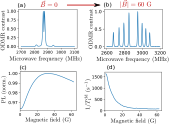
\includegraphics[width=0.9\textwidth]{Figures/scan_1x1x1x1}
\caption{Low field depolarization on sample ADM-150-1 for $\mathbf{B}$ in an arbitrary direction. a) ODMR spectrum for B=0. b) ODMR spectrum for B=60 G. c) PL contrast as a function of the external magnetic field. d) $1/T_1^{\rm dd}$ as a function of the external magnetic field. A $T_1$ measurement was recorded for each magnetic field value and fitted accorded to the protocol described in [REF] with $T_1^{\rm ph}=5\ \rm ms$}
\label{scan 1x1x1x1}
\end{figure}
We will start by showing that NV-NV CR behaves differently in the low magnetic field regime compared to the longitudinal field dominated regime which we studied in the last chapter.

The main issue with studying NV-NV CR in low to zero magnetic field is that there are many competing effects happening simultaneously, with few buttons to adjust in order to isolate each effects.

Fig. \ref{scan 1x1x1x1}-c) and d) show the evolution of the NV PL and stretched lifetime $T_1^{\rm dd}$, defined in the last chapter [REF], as the magnetic field is scanned from 0 to 60 G. The ODMR at the initial and final magnetic fields are shown in Fig. \ref{scan 1x1x1x1}-a) and b).

While it is clear that the spin lifetime as well as the PL increases with the magnetic field, there is no clear indication that this is because of the specificity of the low field region. Indeed, the most likely explanation in this case is that the four classes of NV centers get split apart as the magnetic field increases, which reduces the density of resonant fluctuators for each NV centers. 

We can note however that the PL is not an exact mirror of the spin dynamics: while the low field drop in PL is indeed associated with a reduced spin lifetime, the drop in PL at higher magnetic field comes from the states mixing induced by the transverse magnetic field, and is not associated with a modification of the spin dynamics (to the first order).

\begin{figure}[h]
\centering
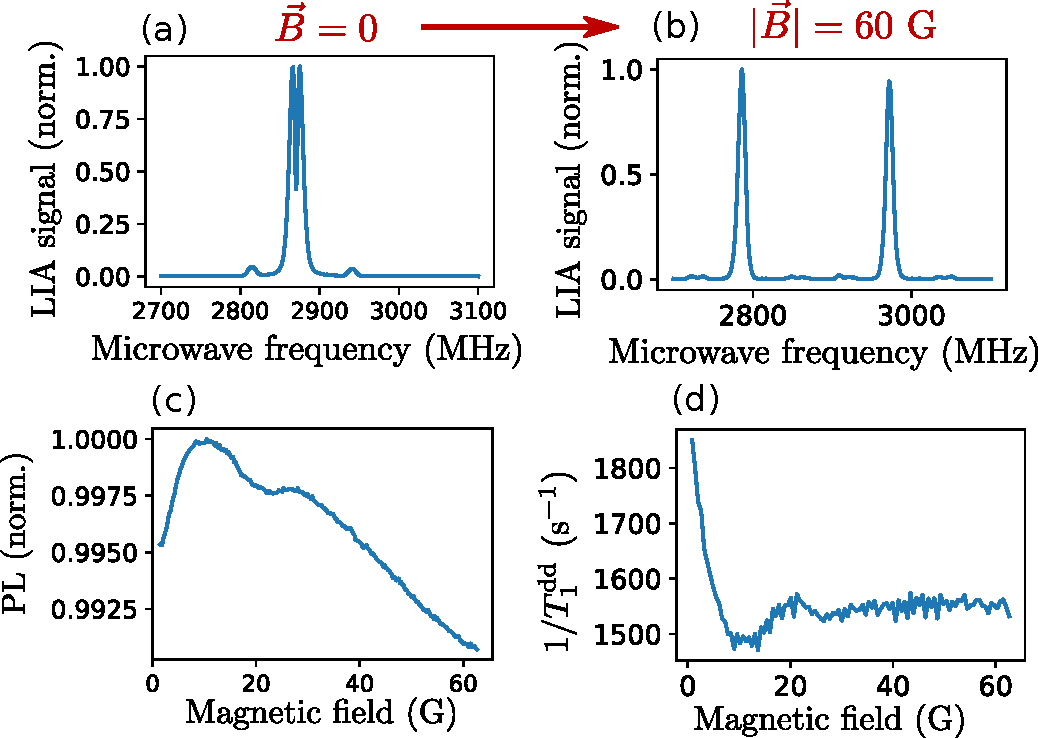
\includegraphics[width=0.9\textwidth]{Figures/scan_100}
\caption{Same measurements as Fig. \ref{scan 1x1x1x1}, still on sample ADM-150-1, but with $\mathbf{B}$ along the [100] axis.}
\label{scan 100}
\end{figure}

Fig. \ref{scan 100} presents a way to circumvent this issue: by applying the magnetic field along the [100] crystalline axis, we can make sure that the four classes of NV centers always stay resonant regardless of the magnetic field amplitude.

We can notice that there still is a decrease of both the PL and $T_1^{\rm dd}$ in low field, although considerably smaller than the previous case: in Fig. \ref{scan 1x1x1x1}, $T_1^{\rm dd}$ was reduced by a factor of $\sim$ 8 in zero field, whereas in Fig. \ref{scan 100}, it was only reduced by a factor of $\sim$ 1.2. The main reason for the PL and $T_1$ drop in Fig. \ref{scan 1x1x1x1} was indeed the co-resonance between the four classes.

Nevertheless, the fact that there is a drop in zero field when $\mathbf{B} \parallel [100]$ cannot be explained if we consider only the inter-class resonances. This means that there are some additional depolarization mechanisms which are proper to the zero field region. We should also note that, while the zero-field PL contrast is bigger in Fig. \ref{scan 1x1x1x1}-c) than in Fig. \ref{scan 100}-c), the PL slope, which is the limiting factor for sensing ability, is actually similar in both cases.

We can also note a drop in PL and a corresponding increase of $1/T_1^{\rm dd}$ for $B \sim 20\ \rm G$ which corresponds to the NV$-^{13}$C-NV cross-relaxation discussed in [REF]

\subsection{Theory of the low field depolarization}
\label{sec causes zero field}
We have identified three possible reasons for the zero field depolarization observed in Fig. \ref{scan 100}. Once presented, we will try to hierarchized the contribution of each of these effects.

\subsubsection{Eigenstates modification}
The first explanation is the modification of the dipole-dipole interaction caused by the change of the NV Hamiltonian eigenbasis from $\{ \ket{0}, \ket{\pm 1} \}$ when $\mathbf{B} \neq 0$ to $\{ \ket{0}, \ket{\pm} \}$ when $\mathbf{B} = 0$.

This modification arise from the new form of the dipole-dipole Hamiltonian in the $\{ \ket{0}, \ket{+}, \ket{-} \} \times \{ \ket{0}, \ket{+}, \ket{-} \}$ basis. We justify this change of basis, where we only considered the single NV Hamiltonian instead of the full two-spins Hamiltonian, by the fact that we are in the weak coupling regime, where $\expval{\mathcal{H}_{dd}} \approx 50\ \rm kHz \ll \frac{1}{2\pi T_2^*} \approx 5\ \rm MHz$ meaning that we can treat the dipole-dipole interaction perturbatively. To compute the decay rate with these new eigenstates, we now need to consider the $\mel{0,\pm}{\mathcal{H}_{dd}}{\pm ,0}$ matrix elements instead of the $\mel{0,\pm 1}{\mathcal{H}_{dd}}{\pm 1,0}$ ones.

The computation of the decay rates in the new eigenbasis involve the averaging of these matrix elements which is detailed in appendix [REF]. The computation in this case is complicated by the fact that the transverse field (either $\mathbf{E}$ or $\mathbf{B}$) responsible for the splitting of the $\ket{\pm}$ levels breaks the Hamiltonian symmetry in the $(xy)$ plane. This means that the dipole-dipole coupling between two spins will depend on their relative $x$ and $y$ axis, defined by the local transverse field, on top of the relative $z$ axis defined by the NV axis. 

We therefore need to make an assumption on the distribution of the transverse field in the sample. In zero external magnetic field where the dominant transverse field comes from randomly spaced charged impurities, we can expect the $x$ and $y$ axes to be randomly sampled in their respective $(xy)$ plane. However, since the NV-fluctuator CR is dominated by the closest neighbor of each spin (due to the $1/r^6$ scaling in eq. [REF]), there could still be local correlations in the transverse field felt by the NV and its nearest fluctuator.

We then computed the decay rates for the two extreme cases: first, we consider that the $x$ and $y$ axis of each spin is randomly sampled, which correspond to a correlation length of the transverse field $l_c=0$, and secondly we considered the case where the dominant transverse field as a fixed orientation in the whole sample corresponding to $l_c=\infty$.

We found for $\mathbf{B}=0$ that the expected decay rate was $\Gamma_1=51.4 \Gamma_0^{\rm th}$ if $l_c=0$ and $\Gamma_1=55.0 \Gamma_0^{\rm th}$ if $l_c=\infty$. $\Gamma_0^{\rm th}$ has the same definition as in table [REF], it is the expected decay rate for an isolated class in the $\{ \ket{0}, \ket{\pm 1} \}$ basis.

In both cases, this is a moderate ($\sim 20 \%$) increase compared to $\Gamma_1=42.8 \Gamma_0^{\rm th}$ which we previously found for $\mathbf{B} \parallel [100]$, where all four classes were degenerate but the Hamiltonian eignebasis was $\{ \ket{0}, \ket{\pm 1} \}$. The change in the Hamiltonian eigenbasis for low field is therefore a possible candidate to explain the low field depolarization in Fig. \ref{scan 100}

\subsubsection{Double flips}

\begin{table}[htbp]
\centering
\caption{Simulated depolarization rate for flip-flops and double flips in zero magnetic field}
 \label{table double flips}
\begin{tabular}{c|cc}
%\toprule
{} & $l_c=0$ & $l_c=\infty$ \\
\midrule
$\bar{R}^2=1$ & $126.8 \Gamma_0^{\rm th}$ & $126.8 \Gamma_0^{\rm th}$ \\
$\bar{R}^2=0.5$ & $93.7 \Gamma_0^{\rm th}$ & $95.4 \Gamma_0^{\rm th}$ \\
$\bar{R}^2=0$ & $51.4 \Gamma_0^{\rm th}$ & $55 \Gamma_0^{\rm th}$ \\
%\bottomrule
\end{tabular}
\end{table}

Another effect which happens only at low magnetic field is the possibility of double flip between the NV center and the fluctuator, which is the simultaneous flip of both spins in the same directions, for example going from $\ket{0,-1}$ to $\ket{+1,0}$. The processes $\ket{0, \pm 1}\bra{\mp 1,0}$ are resonant for $B=0$ and not anymore when the degeneracy between the $\ket{\pm 1}$ states is lifted by the magnetic field.

We have seen however that for weak magnetic fields the eigenstates of each NV Hamiltonian are $\ket{\pm}$ and not $\ket{\pm 1}$, due to the transverse electric field. And the $\ket{+}$ and $\ket{-}$ states are not resonant in zero magnetic field. But we can see from Fig. \ref{simus ESR}-d) or \ref{ESR for T2*}-c) that the splitting $2 d_\perp E_\perp \approx 8\ \rm MHz$ is of the same order than the $1/T_1^{\rm dd}$ profile of linewidth $\Gamma^{\rm dd} \approx 8.8\ \rm MHz$ measured on Fig. [REF]. In zero external magnetic field, the $\ket{+}$ and $\ket{-}$ states are therefore close enough in energy that double flip can take place.

To compute the depolarization induced by the double flips, we need to add another decay channel in the fluctuator model, on top of the flip-flop one. We also need to take into account the fact that the $\ket{+}$ and $\ket{-}$ states are not fully resonant, which will modify the $\bar{R}$ factor defined in [REF]. Finally, the question about the correlation  length of the electric field also needs to be asked.

The results are summed up in Table \ref{table double flips}. We again give the results for the two extreme cases regarding the correlations in the electric field, and we show three possible scenario regarding the pseudo-resonance of the $\ket{+}$ and $\ket{-}$ states, represented by the $\bar{R}^2$ factor: $\bar{R}^2=1$ means that the states are fully resonant ($\omega_+-\omega_- \ll \Gamma^{\rm dd} $), this would be the maximum possible decay rate involving the double flips. $\bar{R}^2=0.5$ represents the case where the splitting between the states is equal to the fluctuator linewidth ($\omega_+-\omega_- \approx \Gamma^{\rm dd}$). This is close to the the experimental values we have. Finally $\bar{R}^2=0$ correspond to the case where the states are too far detuned for the double flips ($\omega_+-\omega_- \gg \Gamma^{\rm dd} $). We come back to the results of the last section where only considered the flip-flops.


\subsubsection{$T_2^*$ modification}

The last aspect we considered was the change in $T_2^*$ (we include the change in the hyper-fine interaction in the $T_2^*$) for weak magnetic field, as discussed in sec. \ref{sec modif T2*}.

To quantify its impact in the depolarization rate, we employ eq. [REF], where we use the values $2\gamma_f = 6.5\ \rm MHz$ estimated in the last chapter and we take for $\Gamma_f=\Gamma_{\rm NV}$ the values of half width at half maximum found in Fig. \ref{ESR for T2*}. 

We then find that the modification of $T_2^*$ should increase the decay rate in zero field by $\sim 9 \%$ for sample Sumi-2, and by $\sim 24 \%$ for sample CVD-pink. 


\subsubsection{Summary}
\begin{figure}[h]
\centering
\includegraphics[width=\textwidth]{Figures/Shema_summary_theory}
\caption{Visual summary of the different depolarization effects in low magnetic field and their predicted depolarization rate}
\label{summary_theory}
\end{figure}

Fig. \ref{summary_theory} recapitulate the various mechanisms at play in the low field depolarization of NV ensemble. 

We start from from the simplest case where every classes are sepctrally isolated and the only dipole-induced relaxation coms from the flip-flop between NV and fluctuators from the same class. We then consider the case where all four classes are resonant ($B\parallel [100]$) and finally the case B=0.

The three extra depolarization mechanisms in zero field are then detailed, with the predicted increase of depolarization rate for each step. The predicted rates in zero field depend on several parameters, we chose the following ones to compute the different numerical values: $l_c=0$, $\bar{G}^2=0.5$, $2\gamma_f = 6.5\ \rm MHz$ and $2/T_2^*=5.9\ \rm MHz$ (corresponding to sample Sumi-2 if we assume a Lorentzian ODMR profile).

\subsection{Other potential causes for zero field depolarization}
We have also considered two other potential causes that we have ultimately ruled out in this case.

\subsubsection{Magnetic field alignment}
\begin{figure}[h]
\centering
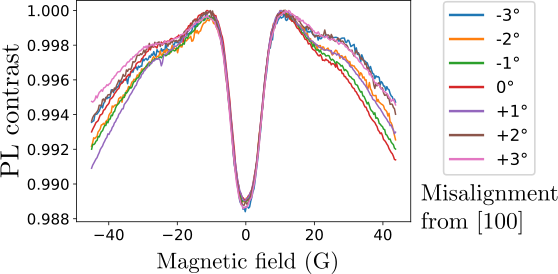
\includegraphics[width=.7\textwidth]{Figures/alignement_rose}
\caption{PL of sample CVD-pink as a function of the magnetic field for various misalignment of the field direction with the [100] axis}
\label{alignement rose}
\end{figure}

The first is a potential misalignment of the magnetic field with the [100] axis, which would cause a splitting of the 4 classes as the magnetic field increases. This hypothesis is not consistent with the observations in Fig. \ref{scan 100}-d): we would expect a small  misalignment to cause a slow but steady decrease of $1/T_1^{\rm dd}$ as the magnetic field is increased. Instead we observe a sharp decrease followed by a pseudo-plateau.

We still estimated how sensitive the PL dip was with respect to the field alignment. Fig. \ref{alignement rose} shows PL scans on sample CVD-pink for various alignment of the magnetic field around the [100] axis. We estimate our alignments to be precise within $\pm 1^\circ$. We can see that the central feature is almost unaffected by the orientation within [$-3^\circ$:$+3^\circ$] which confirms that the low field depolarization does not come from a field misalignment.

\subsubsection{Laser polarization}
\begin{figure}[h]
\centering
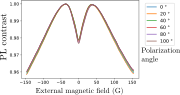
\includegraphics[width=.7\textwidth]{Figures/pola_laser}
\caption{PL of sample ADM-150-3 with respect to the magnetic field for various laser polarization angle. The magnetic field orientation was chosen arbitrarily in the plane of polarization of the laser field}
\label{pola laser}
\end{figure}

Other studies \citep{anishchik2015low, filimonenko2020weak} previously saw a correlation between the zero magnetic field PL dip and the polarization angle of the laser with respect to the magnetic field. 

Fig. \ref{pola laser} shows PL scans on sample ADM-150-3 for various polarization angle of the incident laser. We chose to apply the magnetic field in the laser polarization plane, in a direction that did not match any particular crystalline planes.

We can see no clear differences between the different polarization angles used, whereas \citep{anishchik2015low} and \citep{filimonenko2020weak} saw an antiline growing inside the PL dip when $B \perp E_{\rm las}$. We think that the difference between our experiments come from the fact that we are using denser NV ensembles, and that any effects tied to the laser polarization are hidden by the stronger effects discussed previously.


\section{NV-NV CR under purely transverse magnetic field}
We have seen in the last part that there was a spontaneous spin depolarization specifically in zero external magnetic field, and we have identified three potential mechanisms which are the double-flips, the change in the Hamiltonian eigenstates and the modification of $T_2^*$. We now want to experimentally discriminate the contribution of each of these mechanisms and to see how close the actual decay rates are to the predicted ones. 

One of the reason we want to separate these contributions is that they scale differently with the different variables of the sample ($T_2^*$, $\gamma_f$ , magnetic and electric noise ...). Understanding which of these effect dominates the zero field dynamics might give us insight on which parameter to optimize if one wants to avoid the zero field depolarization, or on the contrary to increase it.

The ideal way to isolate each contributions would be to apply an electric field strong enough to split the transition of the 4 classes, and to measure the decay rate of a single class dominated by the transverse electric field. Such an electric field would need to be of the order of $\sim 10^6\ \rm{V/cm}$, which is several order of magnitudes greater than the breakdown voltage of air and out of our experimental reach.

Instead of an electric field, we will use a transverse magnetic field, which as described in sec. \ref{sec B transverse} leads to a spin Hamiltonian similar to the one where the transverse electric field dominates, or at least to similar eigenstates.

\subsection{Principle of the experiment}
\begin{figure}[h]
\centering
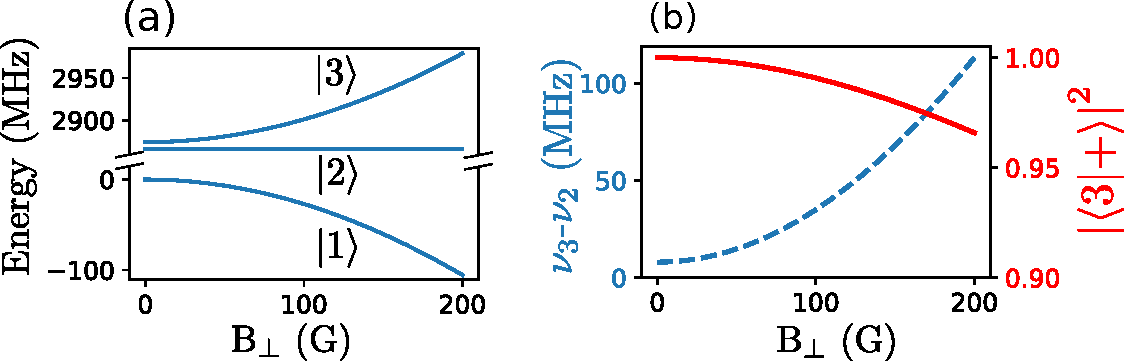
\includegraphics[width=\textwidth]{Figures/transis_transverse_field}
\caption{Simulation of the eigenstates of the NV Hamiltonian for  a purely transverse magnetic field $B_\perp$. In addition to the transverse magnetic field, we consider a fixed transverse electric field of value $d_\perp E_\perp=4\ \rm MHz$. (a) Eigenvalues for the spin Hamiltonian as a function of $B_\perp$. The three states are labeled $\ket{1}$, $\ket{2}$ and $\ket{3}$. (b) Splitting between the $\ket{2}$ and $\ket{3}$ states (blue curve) and closeness factor $\abs{\bra{3}\ket{+}}^2$ between the $\ket{3}$ and $\ket{+}$ (red curve)}
\label{eigenstates transverse field}
\end{figure}

Fig. \ref{eigenstates transverse field} shows a simulation of the eigenstates and eigenenergies for a NV Hamiltonian subject to transverse electric field and magnetic field. For convenience we chose to take $E_\perp = E_x$ and $B_\perp = B_x$, taking other geometric configuration alters only slightly the results. We labeled the eigenstates of the Hamiltonian $\ket{1}$, $\ket{2}$ and $\ket{3}$ in ascending order of energy.

Fig. \ref{eigenstates transverse field}-b) shows both the splitting $\Delta \nu$ between the $\ket{2}$ and $\ket{3}$ states, and how close the $\ket{3}$ state is to the $\ket{+}=\frac{\ket{+1}+\ket{-1}}{\sqrt{2}}$ state via the factor $\abs{\bra{3}\ket{+}}^2$. We look at the $\ket{3}$ state since $\ket{2}=\ket{-}=\frac{\ket{+1}-\ket{-1}}{\sqrt{2}}$ in this case.

These two metrics, $\Delta \nu$ and $\abs{\bra{3}\ket{+}}^2$ are what we are interested in: we want to increase $\Delta \nu$ to the point where the double flips are completely quenched, but we want $\abs{\bra{3}\ket{+}}^2$ to remain close to 1 since we wanted to observe the modification caused by the eigenbasis $\{\ket{0},\ket{\pm}\}$. This way we can isolate the $T_1^{\rm dd}$ contribution coming from the change of eigenstates to the one coming from the double flips. Based on the plots in Fig.\ref{eigenstates transverse field}-b), the region with $B_\perp \in$ [100,200] G seems to satisfy both these criteria.

\subsection{Experimental data}

\begin{figure}[h!]
\centering
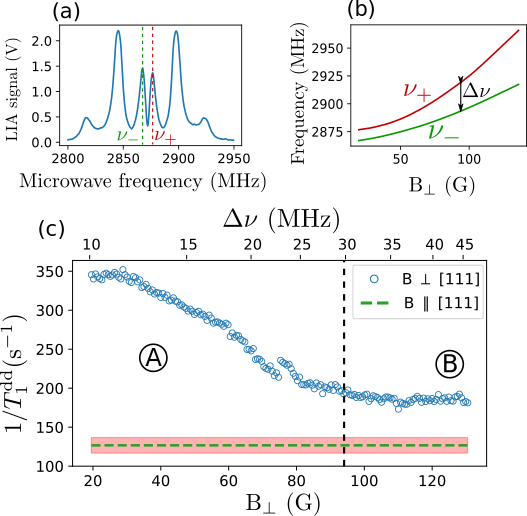
\includegraphics[width=.8\textwidth]{Figures/scan_T1_perp}
\caption{Experimental data for the depolarization under purely transverse magnetic field on sample ADM-150-2. a) ODMR spectrum for $|\mathbf{B}|=20\ \rm G$. The transitions of the class orthogonal to the magnetic field are labeled $\nu_+$ and $\nu_-$. b) Dependency of $\nu_+$ and $\nu_-$ with the magnetic field, as measured through ODMR. c) Measurement of $T_1^{\rm dd}$ as a function of the transverse magnetic field. The corresponding energy splittings $\Delta \nu=\nu_+-\nu_-$ are written on top. We divided the plot between the A region where $1/T_1^{\rm dd}$ decreases, and the B region where it reaches a plateau with a value $1/T_1^{\rm dd}=185 \pm 5\ \rm s^{-1}$ indicated by a red line. We also indicate in green the value found for a purely longitudinal magnetic field $1/T_1^{\rm dd}=126 \pm 10\ \rm s^{-1}$}
\label{champ tranverse exp}
\end{figure}

We perform here a $T_1^{\rm dd}$ measurement similar to the one presented in Fig. [REF], on the same sample and with the same fitting parameters, but this time probing a class orthogonal to the magnetic field.

Fig. \ref{champ tranverse exp}-a) and b) show the evolution of the transition frequencies $\nu_+=\frac{E_{\ket{3}}-E_{\ket{1}}}{h}$ and $\nu_-=\frac{E_{\ket{2}}-E_{\ket{1}}}{h}$ where $\ket{1}$, $\ket{2}$ and $\ket{3}$ are the states described in Fig. \ref{eigenstates transverse field}. The magnetic field was scanned between 20 and 130 G by increment of $\sim 0.5\ \rm G$.

Fig. \ref{champ tranverse exp}-c) shows the evolution of $1/T_1^{\rm dd}$ with the magnetic field. We have denoted two region: in region A, $1/T_1^{\rm dd}$ decreases with the magnetic field, from a value of $350\ \rm s^{-1}$ to a value of $185\ \rm s^{-1}$. In region B, the value of $1/T_1^{\rm dd}$ is stable and does not decrease further when $B_\perp$ is increased.

\subsubsection{Region A}

We attribute the decrease in region A to the double flips: as the magnetic field increases, so does $\Delta \nu$ and the double flips become less and less resonant to the point where they become completely quenched for $B_\perp \approx 90\ \rm G$ or $\Delta \nu \approx 30\ \rm MHz$. This value is coherent with the previously measured fluctuator linewidth. We can then estimate the part of the double flips in the total depolarization rate for the low field regime (20 G here) and find that they amount for $\sim 50\%$ in this case.

Another possibility to explain this drop could be that the class orthogonal to $\mathbf{B}$ still exerts flip-flops with the other classes at low magnetic field, as we can see in Fig. \ref{champ tranverse exp}-a) that they are not very far detuned. However we have to consider that the detuning between the two states $\nu_+-\nu_-= 9\ \rm MHz$ is significantly lower, even at $B_\perp=20\ \rm G$, than the detuning with the closest class $\nu_\pm-\nu_{\rm other}= 22\ \rm MHz$; and also that there seem to be a small plateau for $1/T_1^{\rm dd}$ at the beginning of region A which is consistent with the double flip hypothesis since  $\nu_+-\nu_-$ is almost flat in this region while $\nu_\pm-\nu_{\rm other}$ increases linearly with the magnetic field.

\subsubsection{Region B}

We now turn to region B. Even tough the double flips are completely quenched, the effects of the eigenbasis modification and the $T_2^*$ reduction are still present, because we can see on Fig. \ref{eigenstates transverse field}-b) that the eigenstates of the spin Hamiltonian are still very close to $\{ \ket{0}, \ket{\pm} \}$ for these magnetic field values.

To evaluate the contribution of the eigenbasis and $T_2^*$, we measure the same class of NV centers, but this time with a longitudinal magnetic field ($B_\parallel \sim 100 G$) to get a baseline value of $1/T_1^{\rm dd}$ in the $\ket{\pm 1}$ basis. We found a value of $1/T_1^{\rm dd}=126 \pm 10\ \rm s^{-1}$ in this case, reported on Fig. \ref{champ tranverse exp}-c) as a green line. 

We do find that the decay rate is higher in the $\ket{\pm}$ basis by $\sim 50\% $ which corroborates our predictions, as both the change of eigenbasis from $\ket{\pm 1}$ to $\ket{\pm}$ and the increase of $T_2^*$ in the $\ket{\pm}$ basis are predicted to increase the depolarization rate. The theoretical increase however overestimates once again the actual increase: for the change of eigenbasis alone we predicted an increase of the decay rate by a factor of 4 (see appendix [REF]), over 8 times more than the actual increase.

We unfortunately cannot experimentally discriminate the depolarization coming from the eigenbasis change or the $T_2^*$ while using the same sample, since both of this properties are tied to the Hamiltonian eigenstates. But we do know that in this scenario, for a single isolated class, the contribution of both the change of eigenbasis and $T_2^*$ amounts for $\sim 3$ times less than the double flips. 

\subsubsection{Conclusion of the experimental observation}

We have here quantitatively measured different depolarization contributions for a single class submitted to purely transverse magnetic field, and we expect that the depolarization for low magnetic fields behave similarly. We therefore claim that the difference in NV polarization between the $\mathbf{B}=0$ region and $\mathbf{B} \neq 0$ region is caused by (in order of importance):
\begin{enumerate}
\item The lift of degeneracy between the four classes caused by the projection of the magnetic field on the different NV axis.
\item The double flips between the nearly resonant $\ket{+}$ and $\ket{-}$ states at low magnetic field.
\item The change of the Hamiltonian eigenbasis from $\{\ket{0}, \ket{\pm} \}$ in the electric field dominated region to $\{\ket{0}, \ket{\pm 1} \}$ in the magnetic field dominated region, and the incident change in $T_2^*$.
\end{enumerate}

\section{Introduction to ensemble NV magnetometry}

Before we explore the application of low field depolarization to magnetometry, we must discuss the general field of NV magnetometry. 

NV magnetometry is generally decomposed between single NV and ensemble magnetometry. Single NVs,often associated with scanning probes, offer a spatial resolution limited only by how far the magnetic source can be from the NV center (typically $\sim 10\ \rm nm$), but at the cost of a relatively low sensitivity (typically $\sim \mu \rm{T} / \sqrt{\rm Hz}$ \citep{pelliccione2016scanned}).

Ensemble NV centers center on the other hand offer sensitivities as low as $1\ \rm pT / \sqrt{\rm Hz}$ \citep{wolf2015subpicotesla}, at the cost of working with samples of sizes up to several mm.

We will only focus here on NV ensemble magnetometry since we want to give elements of comparisons with our technique based on NV-NV CR. We will not try to give a complete overview of this field, but only of the elements close to the technique we present. For a general overview on NV magnetometry, we recommend the excellent reviews  \citep{rondin2014magnetometry, degen2017quantum, barry2020sensitivity}.

\subsection{AC and DC magnetometry}
The most sensitive NV magnetometry protocols use the free precession of the spins to map a small change in the Zeeman energy into the phase of the spins, which is then converted into spin population. These protocols are generally distinguished between DC-broadband and AC-narrow band.

For DC-broadband magnetometry, the general technique consist of a Ramsey interferometry experiment, presented in chapter 1, which is limited by the spin inhomogeneous coherence time $T_2^* \lesssim 1\ \rm{\mu s}$ for NV ensembles. The bandwidth of the protocol is limited by the repetition rate of the experiment, generally up to $\sim 100\ \rm kHz$. Although less sensitive in theory, continuous-wave (CW) ODMR and pulsed ODMR are also often employed for DC magnetometry. The state of the art in term of DC ensemble magnetometry is a sensitivity of $\sim 20\ \rm pT/ \sqrt{\rm Hz}$ \citep{barry2016optical, chatzidrosos2017miniature}.

For AC magnetometry, the basic protocol consist of a spin echo measurement, also presented in chapter 1, which extends the coherence time $T_2^*$ to $T_2 = 10 \sim 100 \rm{\mu s}$, and which can be extended even further to $\sim \rm ms$ times with dynamical decoupling \citep{pham2012enhanced}. Due to the longer ``free" precession time, a larger phase can be imprinted on the spin for a similar magnetic field. The AC magnetic field however has to be in phase with the rephasing pulses, which limits the AC sensing to a relatively narrow band. The state of the art in term of AC sensing is $\sim 1\ \rm pT/\sqrt{\rm Hz}$ \citep{wolf2015subpicotesla}.

Recently, \citep{xie2021hybrid} have achieved new records in both DC ($\sim 200\ \rm fT/\sqrt{\rm Hz}$) and AC ($\sim 10\ \rm fT/\sqrt{\rm Hz}$) NV magnetometry by using flux concentrators which are ferromagnets concentrating the magnetic field in a small volume, similarly to an electromagnet. Because the gain from the flux concentrators is not tied to a specific magnetometry protocol, we will focus on the results obtained without flux concentrators.
\subsection{Low field magnetometry}
Magnetometry for low magnetic field ($\gamma B < d_\perp E_\perp$) is challenging since in this regime the NV eigenstates and eigenenergies do not depend on the magnetic field in the first order. This complication is often lifted  by simply using a bias magnetic field, typically from a permanent magnet. 

Some systems however need to be kept under low to zero external magnetic fields, for example to study the J-coupling between spins \citep{sutter2012computational}, or the phase of skyrmions \citep{zazvorka2020skyrmion}. To study these systems with NV centers, we need to find new protocols for low field NV magnetometry.

The main technique for low field magnetometry consist in using circularly polarized microwaves, which can only excite the $\ket{0} \to \ket{-1}$ and $\ket{0} \to \ket{+1}$ transitions, even when these states are not the Hamiltonian's eigenstates \citep{mrozek2015circularly, zheng2019zero, lenz2021magnetic, vetter2022zero}. The best sensitivity achieved with this technique was $250\ \rm pT/\sqrt{\rm Hz}$ \citep{zheng2019zero}.

Another technique consist in using the $^{13}\rm{C}-$NV complex we discussed in sec. [REF] which because of the magnetic field offset caused by the $^{13}\rm{C}$ nucleus are frist order sensitive to the magnetic field even in zero external magnetic field \citep{wang2022zero}. With natural abundance $^{13}\rm{C}$ however, this means that only $\sim 3\%$ of the NV centers are used, and increasing the $^{13}\rm{C}$ concentration can lower the coherence of the NV centers. This technique is more suited for a carefully chosen single NV center.

\subsection{Microwave-free magnetometry}
All the precedent magnetemetry protocols described relied on the use of a controllable magnetic field, to coherently manipulate the NV spin state and to measure the phase imprinted by the magnetic field in the rotating frame.

There are other protocols which correlate the magnetic field with the spin $T_1$ time (relaxometry). These protocols can operate without microwave field and work for either DC or high frequency AC sensing.

\subsubsection{microwave-less DC magnetometry}
The DC microwave-free protocols rely on sharp feature in the PL for specific magnetic fields around certain cross-relaxations processes or level anti-crossing. Fig. [REF] in chapter 2 show such PL features, in particular the ground state level anti-crossing (GSLAC, simply labeled LAC on the figure), the sharpest of these features.

The GSLAC occurs for a purely longitudinal magnetic field where $\gamma B_z = D$, which corresponds to $B=1024\ \rm G$. In these conditions, the normally bright $\ket{0}$ state and the dark $\ket{-1}$ state become resonant and any residual mixing between these two states (coming from the electric field, the strain or the residual transverse magnetic field) will cause a drop in the NV polarization, and in the PL \citep{broadway2016anticrossing}. 

A protocol based on the GSLAC line has been implemented, first only for longitudinal magnetic field measurement \citep{wickenbrock2016microwave} and then for 3D vector measurement \citep{zheng2020microwave} with a sensitivity $\sim 300\ \rm pT/\sqrt{\rm Hz}$.

Another DC microwave-less protocol was proposed based on NV-NV CR \citep{akhmedzhanov2017microwave, akhmedzhanov2019magnetometry}. This technique reconstructs the external magnetic field by scanning an other magnetic field, similar to Fig. [REF] in chapter 3, and by measuring the position of the NV-NV CR lines. By scanning the magnetic field in different directions, one can then recover the initial 3D magnetic field. The author of this paper did not measure the sensitivity of this protocol, but they predict a shot noise limited sensitivity of $24.7\ \rm nT/\sqrt{\rm Hz}$.

\subsubsection{microwave-less AC magnetometry}
The AC microwave-less protocols rely on a direct excitation of the $\ket{0} \to \ket{-1}$ or $\ket{0} \to \ket{+1}$ transitions by the magnetic field probed. The detection bandwidth is adjusted with an external DC magnetic field to bring the NV transitions in resonance with the field probed, which has been implemented from $\sim 10\ \rm MHz$ to $27\ \rm GHz$ \citep{magaletti2022quantum}.

Sensitivities as low as a few $\rm pT/\sqrt{\rm Hz}$ have been recorded near 2.87 GHz \citep{wang2022picotesla, alsid2022solid}, but both protocols are not microwave-free as they rely on a secondary controllable microwave field (either for an heterodyne detection or to add additional pulses).

\subsection{Orientation-free magnetometry}
Every protocol described so far requires a precise knowledge  of the Larmor frequency between the $\ket{0}$ and $\ket{\pm 1}$ states as a function of the magnetic field. This knowledge implies that the direction of each NV axis in the frame of the magnetic field is known, because of the strong anisotropy in the NV Hamiltonian. 

For a single crystal, these axes can always be calibrated through ODMR. However, for a polycrystalline diamond, diamond powder or even a single diamond with an erratic motion, the knowledge of these axes is not possible. New protocols need to be found if one wants to perform magnetometry with these materials.

To our knowledge, the only known orientation-free protocol for DC magnetometry is to use the change in PL caused by the transverse field, which is a property that depends only weakly on the field orientation, especially with an ensemble of NV centers with multiple axes. This protocol however has an extremely low sensitivity and only had marginal use so far\citep{rondin2012nanoscale, tetienne2012magnetic, chapman2013background, jones2020selective}.

Orientation-free magnetometry can also be performed for noise sensing, provided that that the noise is sufficiently broadband to directly excite the NV transitions regardless of their Larmor frequencies. The noise can be probed either by measuring the spin $T_1$ time \citep{kolkowitz2015probing, andersen2019electron} (which does not require a knowledge of the Larmor frequency), or via the PL \citep{finco2021imaging}.

\section{Low field depolarization magnetometry}
\label{sec LFDM}
We will now present and characterize the low field depolarization magnetometry (LFDM) protocol which rely on the spontaneous depolarization of dense NV ensemble at low magnetic field. This protocol works for DC or slowly varying ($\lesssim 10\ \rm kHz$) magnetic field, is microwave-free, orientation-free, and operates at low magnetic field, although a small additional field is required to improve performances.

We will first describe its operation and characterize it before comparing it to the previously mentioned NV magnetometry protocols.

\subsection{Principle of the experiment}

\begin{figure}[h!]
\centering
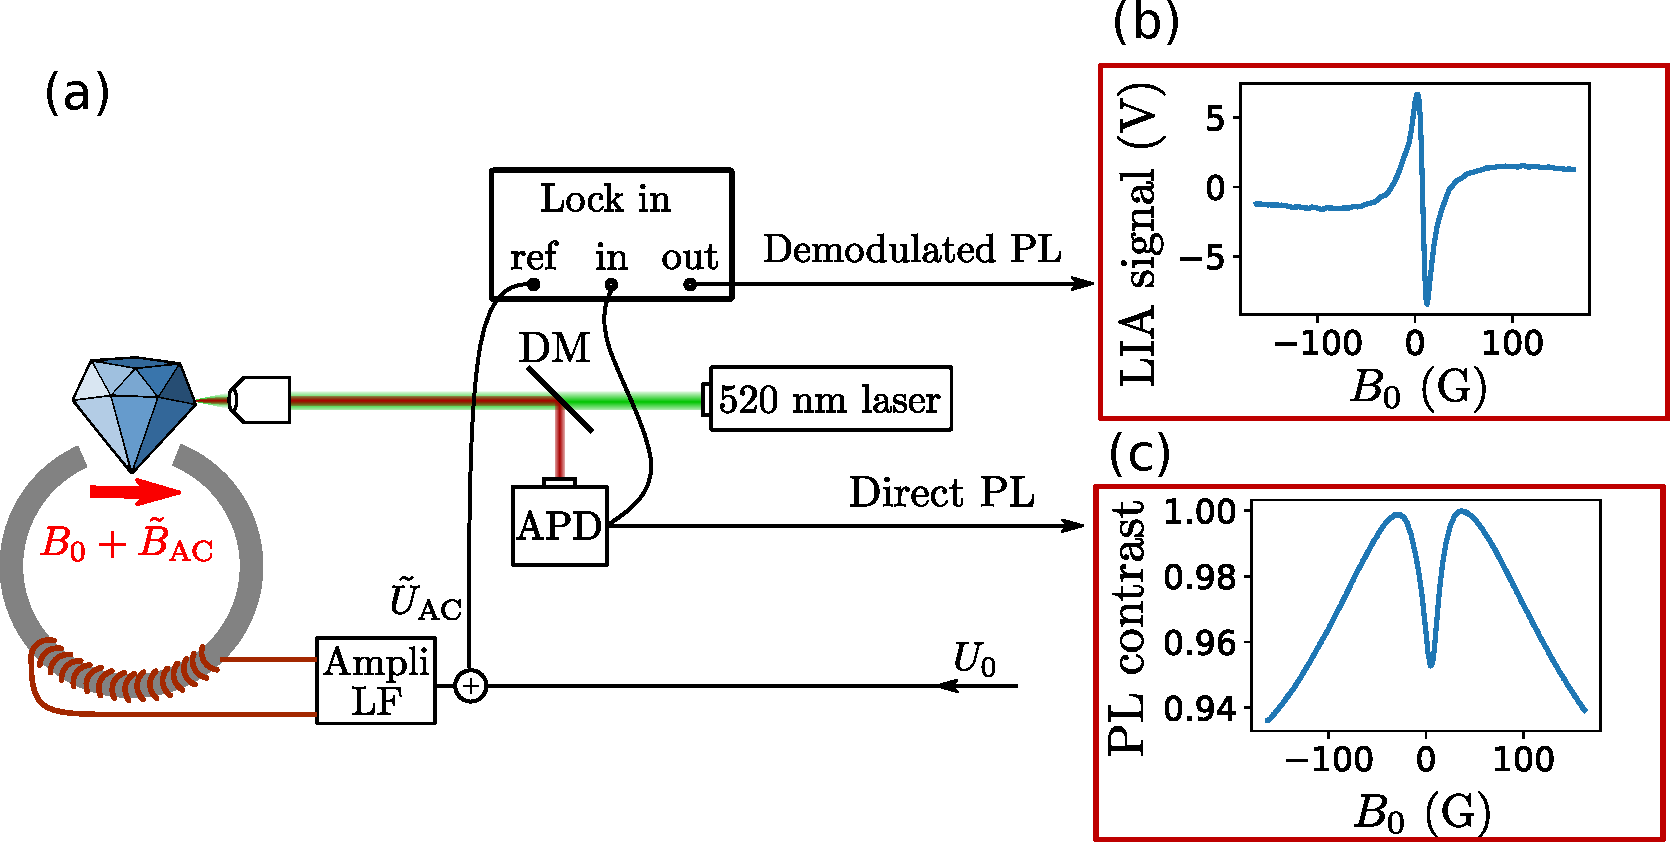
\includegraphics[width=\textwidth]{Figures/setup_magneto}
\caption{Principle of the LFDM protocol a) Experimental setup. The confocal microscopy setup is similar to the one described in [REF], the lock-in amplifier (LIA) is used here to add a modulation on the magnetic field, instead of the microwave. Both the PL and the LIA signal are monitored. b) example of LIA signal on sample ADM-15-4 when scanning the magnetic field $B_0$ between -150 and 150 G. c) PL signal corresponding to the LIA signal}
\label{setup magneto}
\end{figure}

Fig. \ref{setup magneto} shows the principle of the LFDM protocol. The experimental setup is similar to the one presented in Fig. [REF] with the exception that there are no microwaves, and that the magnetic field generated by the electro-magnet contains both a DC or slowly variable component $B_0$ and an oscillating component $\tilde{B}_{\rm AC}$ used for the modulation. We typically use a modulation frequency $f_{\rm mod} \approx 1\ \rm kHz$, the same value we use for ODMR measurements. The main voltage $V_0$ responsible for the DC field and the oscillating voltage $\tilde{V}_{\rm AC}$ responsible for the AC field are summed via a homemade bias tee.

Fig. \ref{setup magneto}-b) and c) show respectively the PL measured directly on the photodiode and the lock-in signal when the DC magnetic field is slowly varied ($f_{\rm scan}<1\ \rm Hz$) from -150 to +150 G. For this configuration, the magnetic field was randomly oriented with respect to the NV axes and did not match any particular crystalline axis.

Both AC (up to $\sim$ 10 kHz) and DC-magnetometry are possible with this setup. To improve the sensitivity however, an AC field needs to be added for the DC sensing, and inversely a DC field needs to be added for the AC sensing. Both of these added fields are typically of a few G for optimal performances, which limits the ultra-low field applications.

\begin{figure}[h!]
\centering
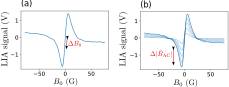
\includegraphics[width=0.9\textwidth]{Figures/AC_and_DC_sensing}
\caption{DC and AC LFDM sensing protocols on sample ADM-15-5. The magnetic field is scanned in an arbitrary direction. a) DC sensing: $B_0$ is scanned between $-$80 and +80 G while an AC field of amplitude 10 G is used for the lock-in detection. b) AC sensing: $B_0$ scans are performed for 5 different $|\tilde B_{\rm AC}|$ values between 2 and 10 G. The best AC sensitivity is achieved for $B_0\approx 5\ \rm G$.}
\label{AC and DC sensing}
\end{figure}

Fig. \ref{AC and DC sensing} shows how the AC and DC sensing work for LFDM: for DC sensing the LIA signal around $B_0=0$ provide a sharp linear slope to convert the LIA voltage into a magnetic field. For AC sensing, the LIA signal is directly proportional to the amplitude of the field. The optimal AC field amplitude for DC sensing has to match the width of the PL dip $|\tilde{B}_{\rm AC}| = \sigma \approx 10\ \rm G$ in order to maximize the slope of the lock-in signal around $B_0=0$. the optimal DC field to use for AC sensing is $B_0= \sigma/2$ corresponding to the region where the lock-in signal is most sensitive to AC field. 

\subsection{Sensitivity of the LFDM protocol}
\begin{figure}[h!]
\centering
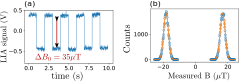
\includegraphics[width=\textwidth]{Figures/sensi_alternee}
\caption{Sensitivity measurement of the LFDM on sample ADM-15-4. a) Temporal trace of the LIA signal when applying an alternating external magnetic field of amplitude 35 $\mu$T and frequency $f=1\ \rm Hz$. b) Histogram of the DC measurement over 50 s. The data is fitted with Gaussians of width $1.6\ \rm{\mu T}$.}
\label{sensei alternee}
\end{figure}

We will now look at the performances of the LFDM protocol before comparing it to the other magnetometry protocols. The characterization was only done for DC sensing. The samples used for the characterization were 15 $\mu$m micro-diamond bought as is from Adamas nanodiamond (see the sample section [REF] for more information).

We characterize the DC sensitivity by looking at the noise floor on the LIA signal when sitting on the steepest slope, around $B_0=0$. The following parameters were used in the case presented: the AC field for the modulation had an amplitude $|\tilde{B}_{\rm AC}|\approx 10\ \rm G$ and a frequency $f_{mod} \approx 1\ \rm kHz$, the laser power was $\approx 1\ \rm mW$ and the collected PL power $\approx 1\ \rm{\mu W}$, and the lock-in low-pass filter time constant was set to $\tau=3\ \rm ms$.

Fig. \ref{sensei alternee} shows the sensitivity measurement protocol. First, the applied magnetic field is calibrated with ODMR spectra, then an alternating DC field of known amplitude (here $\Delta B_0=35\ \rm{\mu T}$) is applied on the sample. Fig. \ref{sensei alternee}-a) shows the temporal trace of the LIA signal in response to this alternating DC field. Knowing the amplitude of the alternating field, we can then convert the voltage signal into a magnetic field amplitude, with in this case a ratio $45 \pm 3\ \rm{\mu T /V}$.

Fig. \ref{sensei alternee}-b) shows an histogram of the measured magnetic field amplitude for both the high and low value of the applied magnetic field. The total acquisition time was 50 s with the external field being alternated every second. The histograms are nicely fitted with Gaussian profiles of width $\sigma=1.5\pm 0.1\ \rm{\mu T}$ which allows us to estimate the DC sensitivity of the protocol:
\begin{equation}
\eta = \frac{\sigma}{\sqrt{2 \tau}}= 116 \pm 10\ \rm{nT} / \sqrt{\rm Hz},
\end{equation}

where $\tau=3\ \rm ms$ is the LIA low-pass filter time constant. 

We estimate that the sensitivity is mostly shot-noise limited because the same LIA voltage noise ($\delta V \approx 35\ \rm mV$) was observed on a magnetic insensitive region (for $B_0 \approx 100\ \rm G$), and is far above the electrical noise measured when no optical signal is sent to the photodiode ($\delta V < 1\ \rm mV$). Laser fluctuations could also play a role but the noise seem to grow as the square root of the optical power and not linearly with it.

\subsection{Angular dependence of the sensitivity}
\label{sec angular sensi}
\begin{figure}[h!]
\centering
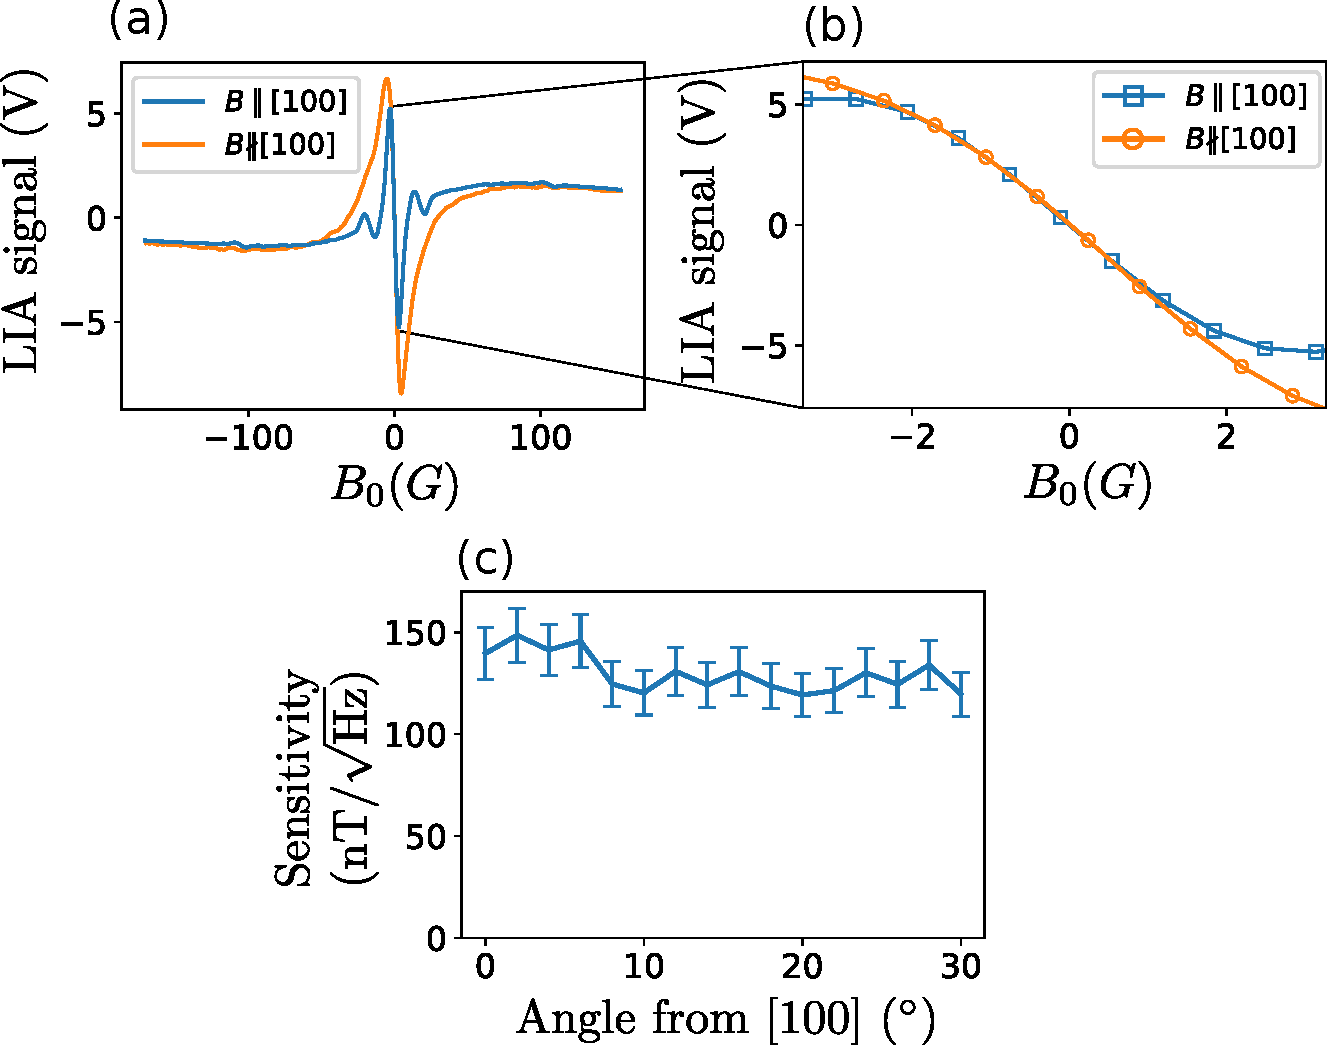
\includegraphics[width=\textwidth]{Figures/sensi_angulaire}
\caption{Angular dependence of the sensitivity. a) LIA signal for $B_0$ scanned between $-$150 and +150 G along the [100] axis, or along a direction 20$^\circ$ off the [100] axis. b) Zoom-in of the LIA signal on the zero-field slopes. c) Measured sensitivity as a function of the magnetic field angle with the [100] axis.}
\label{angular sensi}
\end{figure}

We will now look at the dependence of the sensitivity with respect to the magnetic field angle. In particular, we are interested in comparing the sensitivity when $\mathbf{B}\parallel [100]$, where there is no lift of degeneracy between the four classes as $\mathbf{B}$ increases; and a case where $\mathbf{B}\nparallel [100]$ and where there is a lift of degeneracy between the four classes. We previously saw in Fig. \ref{scan 1x1x1x1} and \ref{scan 100} that the PL and $T_1$ contrast was much smaller when $\mathbf{B}\parallel [100]$, but we now focus on the sensitivity which is related to the slope of the PL change, and not directly to the contrast.

Fig. \ref{angular sensi}-a) and b) show the LIA signal when the DC field $B_0$ is scanned from $-150$ G to +150 G on the same sample ADM-15-4, but for two different angle of $B_0$. For the blue curve, the field was scanned along the [100] axis, for the orange curve, it was scanned with an angle of $\sim 20\ ^\circ$ compared to the [100] axis. We can see that the maximum amplitude of the lock-in signal (relevant for AC sensing) is of the same order of magnitude for both case, and the slope around $B_0$ (relevant for DC sensing) is almost identical. Fig. \ref{angular sensi}-c) shows the sensitivity, measured with the protocol described in Fig. \ref{sensei alternee}, with respect to the angle between the magnetic field and the [100] axis. We can notice that the sensitivity depends only weakly on the magnetic field angle. 

The fact that the sensitivity is similar when $\mathbf{B}\parallel [100]$ or $\mathbf{B}\nparallel [100]$ means that the inter-class co-resonances plays a lower role in the sensitivity than the zero-field specific depolarization mechanisms, previously detailed in Sec. \ref{sec causes zero field}. We cannot be sure which of the three zero-field mechanism is the dominant one, but based on the experimental results shown in Fig. \ref{champ tranverse exp}, we can assume that the double-flips are the dominant factor in the LFDM sensitivity.

It should be noted that this low angular dependence was particularly marked on sample ADM-15-4. Other samples, including from the same batch, showed a higher angular dependence with typically a sensitivity $2 \sim 3$ times worse for $B\parallel [100]$ than for the other directions.

\subsection{Temporal stability}
\begin{figure}[h!]
\centering
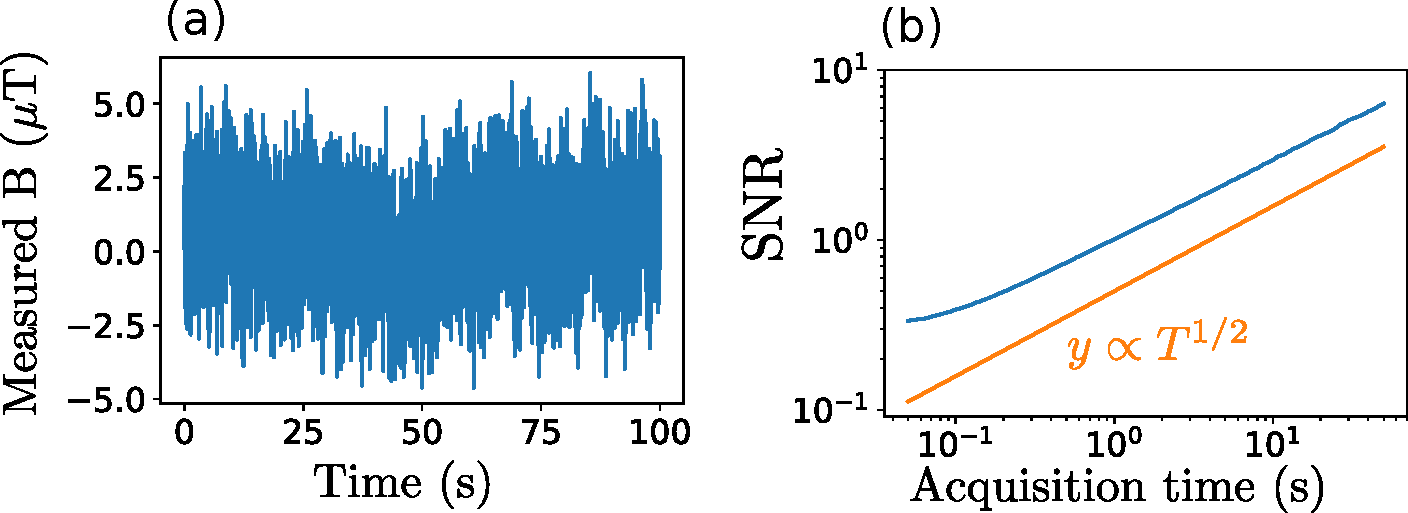
\includegraphics[width=\textwidth]{Figures/Temporal_just_0B}
\caption{Temporal stability of DC-LFDM as measured on sample ADM-15-5. a) Temporal trace of the LIA signal for $B_0 \approx 0$. The Lock-in signal was converted to a measured magnetic field with the previously described protocol. b) Estimated signal to noise ratio for a signal of 100 nT as a function of the total acquisition time $T$. The noise value is computed by averaging the variance of the temporal trace over each time duration $T$. A curve $y=0.5\, T^{1/2}$ is added for comparison}
\label{temporal 0B}
\end{figure}

An important aspect of sensors is their stability in time. The sensitivity being expressed in $\rm{nT} / \sqrt{\rm Hz}$ suggests that the signal to noise ratio (SNR) given by repeating the measurement increases as $\sqrt{T}$ where $T$ is the total acquisition time. This is true for an ideal system, but in practice drifts and low frequency noise mean that the actual SNR for long acquisition time will be worse than the SNR at short time scaled by a factor $\sqrt{T}$.

One of the main source of drift for NV magnetometry based on spin resonance is the crystal lattice temperature change: the $D$ factor in the NV Hamiltonian (eq. [REF]) is sensitive to the lattice temperature because of the thermal dilatation of the crystal, which is the basis for NV thermometry \citep{kucsko2013nanometre}. This means that thermal fluctuations will impact the Larmor frequency of the spins and may cause a detuning with the initial measured frequency for long acquisition times. The LFDM protocol however does not rely on a specific resonance frequency, but rather on a co-resonnance condition between neighboring spins, which does not depend directly on the crystal temperature.

Fig. \ref{temporal 0B} shows the temporal stability of the LFDM protocol over an acquisition time of 100 s. Fig. \ref{temporal 0B}-a) shows a temporal trace of the LIA signal where we have converted the signal into a measured magnetic field. Fig. \ref{temporal 0B}-b) shows the estimated SNR for a signal of 100 nT as a function of the total acquisition time and was computed from the temporal trace.

We can see that the SNR does not deviate from the $\sqrt{T}$ scaling for times up to 50 s, and could probably be extended for longer times. The non-linearity for shorter times comes from the LIA low-pass filter.

\section{Comparison between LFDM and other magnetometry protocol}
Now that we have characterized the LFDM protocol, we can compare its performances with the previously mentioned magnetometry protocols. We should start by mentioning that the best sensitivity achieved with the LFDM ($\sim 100 \rm{nT} / \sqrt{\rm Hz}$) is about $10^5$ times worse than the best NV ensemble sensitivity. This discrepancy however come in large part to the smaller sensor volume used in the characterization, and to a relatively low PL collection efficiency compared to the other experiments.

\subsection{Comparison with microwave based protocols}

\begin{table}[htbp]
\centering
\caption{Comparison of the volume-normalized sensitivity of the best AC and DC protocols with LFDM}
 \label{table sensi volumiques}
\begin{tabular}{c|ccc}
\toprule
{} & Zhou et al. \citep{zhou2020quantum} (AC) & Barry et al.\citep{barry2016optical} (DC) & LFDM (DC) \\
\midrule
$\eta\ (\rm{nT} / \sqrt{\rm Hz})$ & 92&0.015& 116 \\
$V\ (\mu \rm{m}^3)$ &$8.1 \cdot 10^{-3}$ &$5.2 \cdot 10^{6}$& $3.3 \cdot 10^{3}$ \\
$\eta_v\ (\rm{nT}\mu \rm{m}^{3/2} \rm{Hz}^{-1/2})$ &8.3&34&6700 \\
\bottomrule
\end{tabular}
\end{table}

We will first compare the LFDM protocol with the best microwave-based NV magnetometry protocols. A better metric than the sensitivity to compare different protocols is the volume-normalized sensitivity defined in \citep{zhou2020quantum} as $\eta_v=\eta\cdot \sqrt{V}$ where $\eta$ is the sensitivity and $V$ the effective volume of the sensor. This scaling assumes that each NV center in an ensemble is an independent magnetic field probe, and as the total number of NV centers is proportional to $V$, the sensitivity should scale as $1/\sqrt{V}$.

Table \ref{table sensi volumiques} reports the best AC and DC volume-normalized sensitivities found in the literature. The LFDM protocol performs $\sim 200$ times worse than the best DC magnetometer. It should be noted however that the PL collection in our measurement, where we use a confocal microscope with a numerical aperture NA=0.65, is estimated to be $\sim 1 \%$ \citep{le2012efficient}, while the best collection schemes \citep{le2012efficient,wolf2015subpicotesla,wang2022picotesla, alsid2022solid} achieve a collection efficiency above 50 \%.

\begin{figure}[h!]
\centering
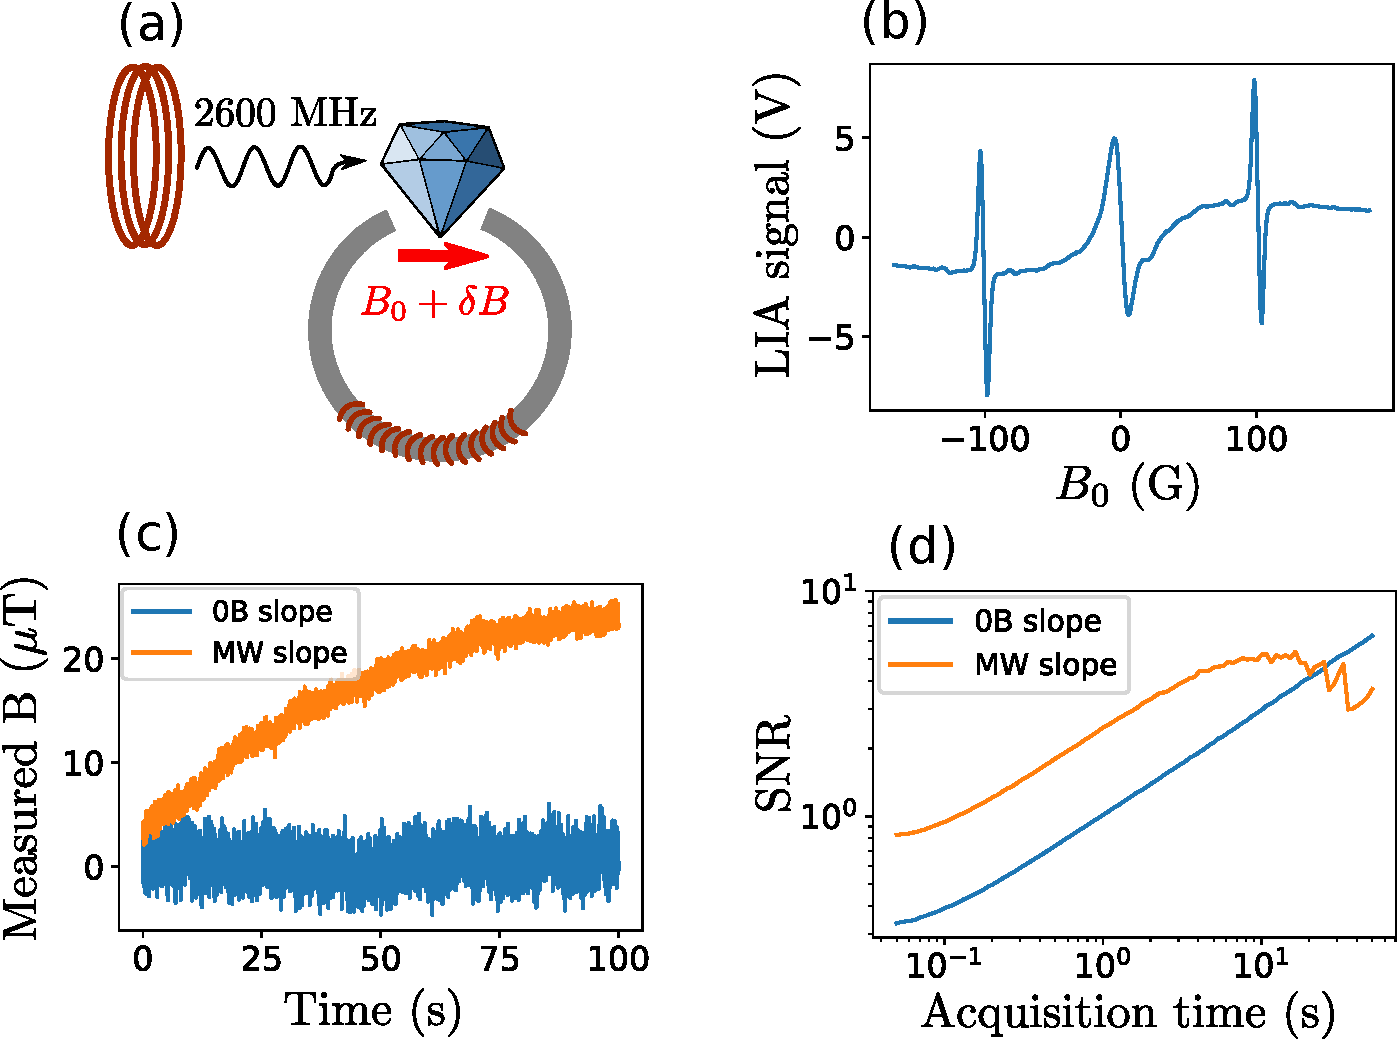
\includegraphics[width=\textwidth]{Figures/compariason_0B_MW}
\caption{Comparison between LFDM and microwave-based magnetometry on the same experimental setup. The sample used is ADM-15-5 and the magnetic field is aligned close to a [111] axis. a) Schematics of the experiment: the setup is the same as the one described in Fig. \ref{setup magneto} with the addition of a continuous microwave tone at the frequency $\nu=2600\ \rm MHz$. b) LIA signal as $B_0$ is scanned from $-$150 to +150 G. The two lines at $\pm 100\ \rm G$ are caused by the microwave. c) Temporal trace of the measured B field for $B_0 \approx 0$ (on the middle of the zero field slope) and $B_0 \approx 100\ \rm G$ (on the middle of the microwave slope). The orange curve is shifted by $\approx 100\ \rm G$ to sit on the same scale as the blue curve. d) Estimated SNR fo a signal of 100 nT for $B_0 \approx 0$ and $B_0 \approx 100\ \rm G$ as a function of the total acquisition time}
\label{comparaison 0B MW}
\end{figure}

Fig. \ref{comparaison 0B MW} shows a comparison between LFDM and microwave-based magnetometry using our setup. A fixed microwave tone (here at 2600 MHz) is sent to the diamond and a magnetic field $B_0$ close to the [111] axis is scanned along an oscillating field $\delta B$ to perform a lock-in detection. 

Fig. \ref{comparaison 0B MW}-b) shows the LIA signal over a $B_0$ scan: the profile is similar to the one in Fig. \ref{setup magneto}-b) with the addition to two sharp lines for $|B_0| \approx 100\ \rm G$. These two lines correspond to the transition $\ket{0} \to \ket{-1}$ (or $\ket{0} \to \ket{+1}$ for the negative fields) of the class aligned with the magnetic field when it comes to resonance with the 2600 MHz microwave tone. The microwave power used here correspond to a Rabi frequency $\Omega \approx (2\pi) 3\ \rm MHz$ and the slope on the steepest part of the microwave line is $\sim 2.5$ times higher than the slope in zero field.

Fig. \ref{comparaison 0B MW}-c) and d) show the temporal stability of the sensor similarly to Fig. \ref{temporal 0B}, on both the zero field line and the microwave line. While we can see that the microwave signal is more sensitive thanks to the higher slope, it is also more prone to drift, most likely because of the shift of the Larmor frequency caused by temperature fluctuations. We can even see that the LFDM becomes more sensitive for acquisition times beyond 10 s.

We should acknowledge that this microwave-based detection is not optimal: we are using a technique analogous to CW ODMR which is not as sensitive as Ramsey interference (although CW ODMR was also the technique used in \citep{barry2016optical}), we were limited in the available microwave power (although in this case $\Omega_{\rm Rabi} \sim 1/T_2^*$ which is supposed to be optimal), and the sample used here had a relatively poor $T_2^* \approx 68\ \rm ns$. Nevertheless, this shows that the LFDM protocol is not that far from basic microwave-based magnetometry with the samples and the optical setup used here.

\subsection{Comparison with microwave-less protocols}
The only microwave-less protocols to have measured a sensitivity are the GSLAC protocols described previously \citep{wickenbrock2016microwave, zheng2020microwave}. Unfortunately the sensing volume in this studies is not known, however due to the similarity in our approaches, we should be able to directly compare the physical origin of both protocols, i.e. comparing the zero field PL dip and the GSLAC PL dip.

In Fig. \ref{setup magneto}-c) we can observe a PL dip with a contrast $C=4.7\pm 1 \% $ for a full width at half maximum $\Gamma=20 \pm 1\ \rm G$. In comparison, in \citep{wickenbrock2016microwave} the authors observe a GSLAC PL dip with a contrast $C=4.5 \%$ for a full width of $12 \ \rm G$ with a type Ib irradiated diamond, similar to the ones we use. In \citep{zheng2020microwave} they manage to keep a contrast of 4.5 \% while reducing the GSLAC linewidth to $0.38\ \rm G$ by using a CVD sample isotopically enriched in $^{12}$C with a lower [NV] and [N] density.

The zero field technique is therefore comparable with the GSLAC technique for samples with high NV and impurity concentration, but unlike the GSLAC magnetometry, it is still unclear what kind of material engineering would improve its sensitivity.

%Je parle pas de la dépendence en puissance ou du champ transverse, je laisse ça pour plus tard.
\section{Conclusion and perspectives}
We have seen in this chapter that dense ensemble of NV centers spontaneously depolarize at low magnetic field, and wee have seen that the depolarization is mediated by dipole-dipole coupling between the NV centers. We have identified three mechanisms by which the depolarization is increased in zero-field: the inter-class flip-flops, the double flips, and the change in the NV eigenstates (which includes the change in $T_2^*$).We have then quantified both theoretically and experimentally the contribution of each of these mechanisms to the zero-field depolarization.

Finally, we have seen how this low-field depolarization can be applied to perform magnetometry experiments, and what advantages and disadvantages this technique offers compared to the established NV magnetometry protocols.

I will now describe what could be interesting investigation points to further improve the LFDM performance, as well as potential applications.

\subsection{LFDM optimization}

Given the few parameters involved in the LFDM protocol, the main path for LFDM optimization seem to be the material optimization of the samples.

Most magnetometry protocols have a relatively clear material optimization path: DC protocols want to improve the figure of merit $\rho T_2^*$ and AC protocols want to improve $\rho T_2$, where $\rho=[\rm NV]$ is the NV concentration. The reason is that the number of NV centers for a given volume scales as $\rho$, and therefore the sensitivity scale as $\sqrt{\rho}$. Meanwhile increasing the density of defects tend to decrease the spin coherence times $T_2$ and $T_2^*$, and the AC and DC sensitivities scale respectively as $1/\sqrt{T_2}$ and $1/\sqrt{T_2^*}$.

For the LFDM protocol however, the material optimization is far from obvious. Indeed, while increasing $T_2^*$ would improve the sensitivity, the gain might not be as interesting as for other protocols due to the broadening caused by the fluctuator lifetime. On the other hand, increasing the NV density not only increases the number of sensor per volume, but also increases the dipole-dipole strength between NV centers. If we assume that fluctuators are constituted of closely packed impurities, then increasing the NV density should also increase the fluctuator proportion.

It seems then that increasing the NV density would be the obvious path to improve the LFDM performances. In practice however, I observed that the relationship between NV density, fluctuators, and LFDM performances was generally not straightforward. The two following examples will illustrate that.

\begin{figure}[h!]
\centering
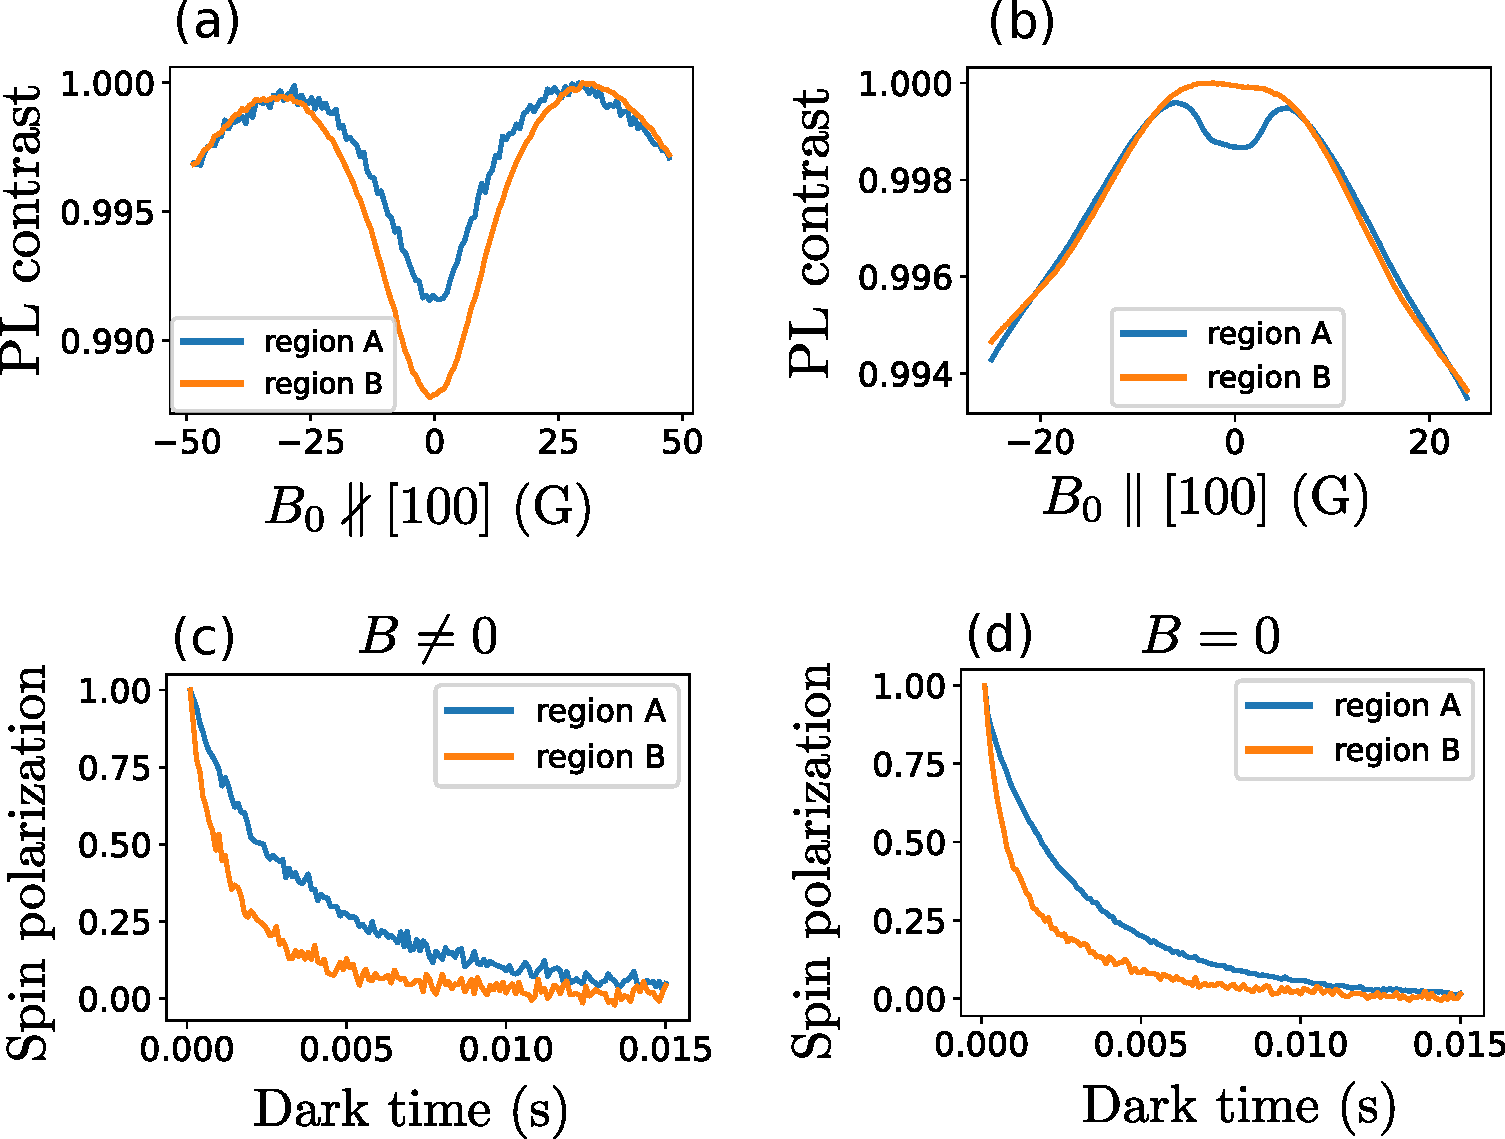
\includegraphics[width=\textwidth]{Figures/substrat}
\caption{Measurements on sample SBST-C for two different regions A and B. a) PL contrast as a function of a magnetic field scanned in an aribitrary direction (same direction for both regions). b) PL contrast as a function of a magnetic field scanned in the [100] direction. c) $T_1$ measurement on a single class when $B\neq 0$. d) $T_1$ measurement on all  four classes when $B=0$ }
\label{substrat chelou}
\end{figure}

Fig. \ref{substrat chelou} shows various measurements on the same sample SBST-C, a HPHT bulk sample containing [NV]$\sim  \rm ppm$, on two spatially distinct regions A and B. These two regions most likely correspond to two distinct growth sectors of the diamond, meaning that these regions were not grown in the same exact environment, which can impact among other things the creation of impurities. Both region showed a similar PL which would indicate a similar density of NV centers.

The metric we are interested in to evaluate the LFDM performance are the PL contrast when $\mathbf{B}$ is scanned in an arbitrary direction, which mainly represents the inter-class flip flop and which I will refer to as FF-contrast; and the PL contrast when B is scanned $\mathbf{B}$ is scanned along the [100] direction, which mainly represents the double flips and which I will refer to as DF-contrast. We are interested in the DF-contrast since we have seen in sec. \ref{sec angular sensi} that it could be the main contribution to the LFDM sensitivity.

Fig. \ref{substrat chelou}-a) and b) indicate that region B shows a higher FF-contrast, but a smaller DF-contrast than region A. Looking at the $T_1$ measurements for both regions, region B shows a shorter $T_1$ in both zero field and non-zero field, which would indicate a larger fluctuator density in region B. If this is true, than the fluctuator density is not directly correlated to the DF-contrast.

\begin{figure}[h!]
\centering
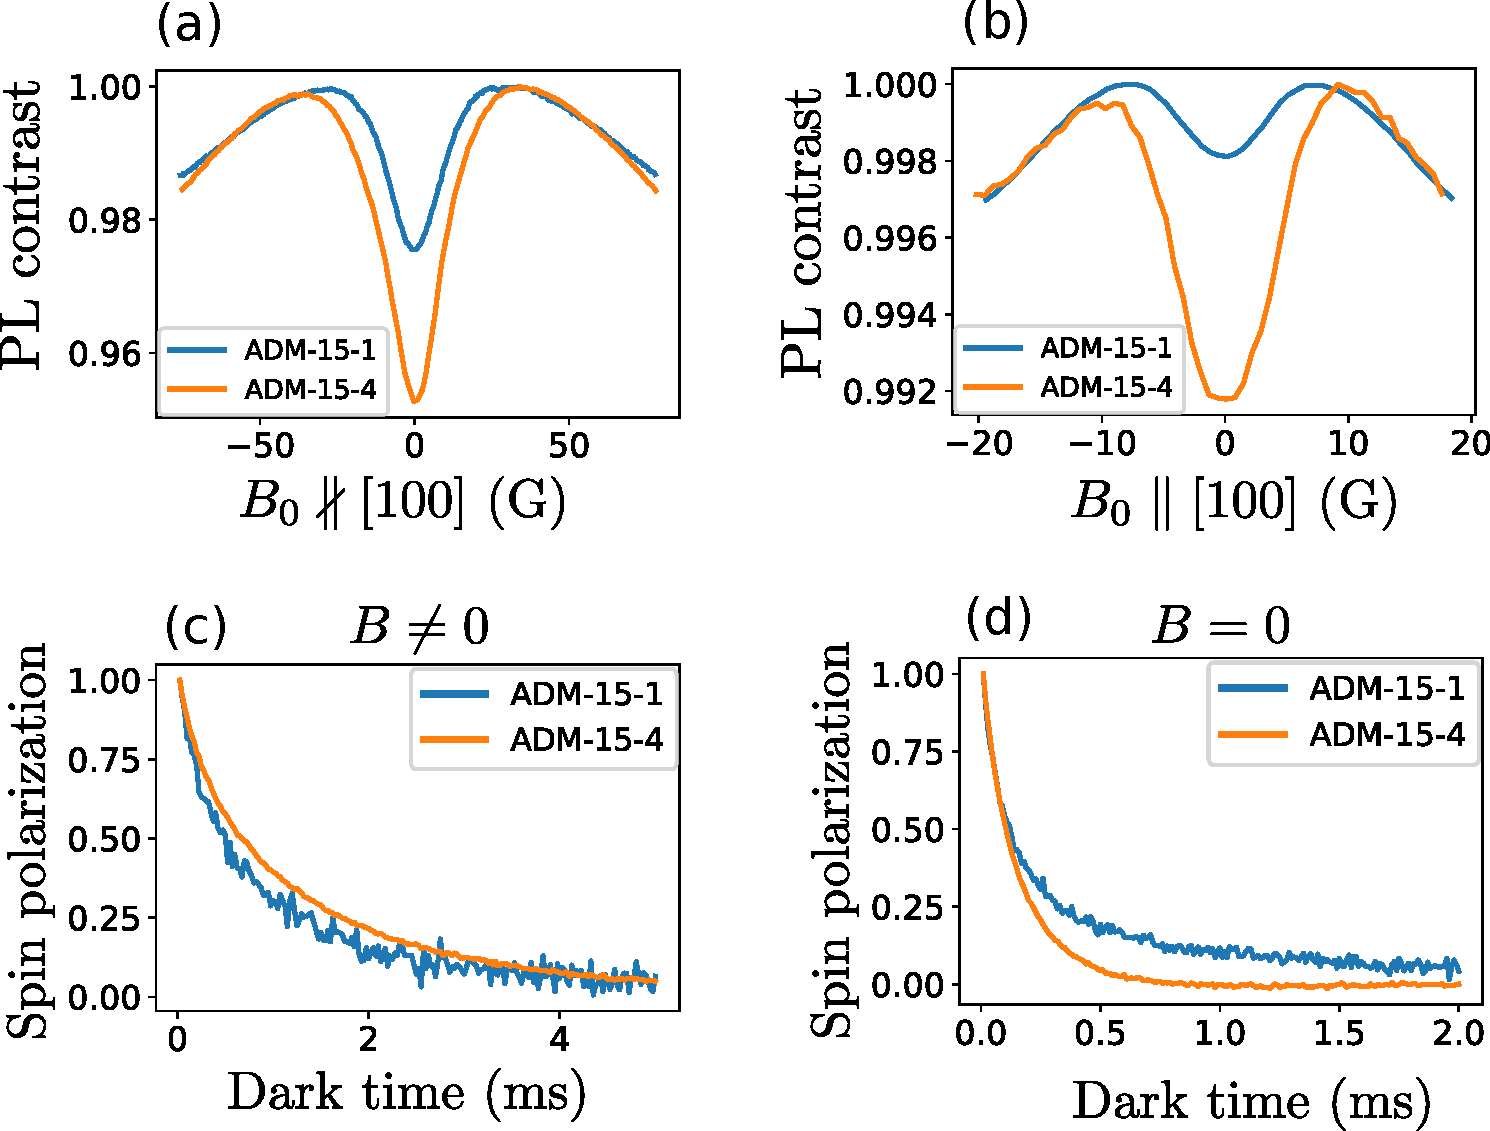
\includegraphics[width=\textwidth]{Figures/double_adamas}
\caption{Same measurements as Fig. \ref{substrat chelou} on two distinct samples ADM-15-4 and ADM-15-1. Every parameters (laser power,optical setup , AC magnetic field) was kept identical for the two samples.}
\label{double dragon}
\end{figure}

We now turn to Fig. \ref{double dragon}. This figure shows the same 4 measurements but this time on two distinct samples, ADM-15-1 and ADM-15-4, which came from the same batch. Both samples showed relatively similar PL which could again indicate a similar NV density.

We can first notice the disparity in the  zero field PL contrasts: the FF-contrast is twice as big in sample ADM-15-4 as in sample ADM-15-1, and the DF-contrast is almost 5 times bigger. When looking at the $T_1$, we can notice that the lifetime for non-zero field is slightly longer for sample ADM-15-4 than for ADM-15-1, but its lifetime in zero-field is shorter (it is also exponential and not stretched-exponential as discussed in the last chapter [REF], which could have an influence on the PL contrast). From the $T_1$ measurements we can not determine which sample contains the most fluctuators, and therefore correlate the fluctuator or NV density with the DF and FF-contrasts.

These two examples illustrate the complexity of finding the sample-dependent parameters that governs the PL contrasts in zero field. We have noticed a large variability in PL contrasts among sample grown in similar condition, which would indicate that those parameters are quite sensitive. If these parameters were to be identified, samples with dedicated fabrication process could then substantially improve the LFDM sensitivity.

Other non-material parameters in the LFDM protocols should also be investigated. This includes the temperature of the sample, the intensity and wavelength of the laser, the frequency and amplitude of the AC magnetic field. For the results presented in sec. \ref{sec LFDM}, we chose the parameters which we found optimal within our available experimental range.


\subsection{Potential applications for LFDM}

\begin{figure}[h!]
\centering
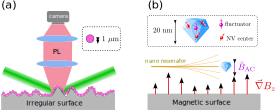
\includegraphics[width=\textwidth]{Figures/Applications}
\caption{Schematics of two potential application for LFDM. The working of each application is detailed in the main text}
\label{applications}
\end{figure}

We will now turn to potential applications for LFDM, which could be useful even without material optimization.

Fig. \ref{applications} illustrates two potential applications for LFDM. The first one is to to perform wide-field magnetic imaging on a surface with micron-sized irregularities. The current leading technology for wide field imaging is to use a bulk CVD diamond with a very well polished surface in direct contact with the probed sample \citep{levine2019principles, scholten2021widefield}. While the diamond surface can be controlled within a few nm, the same is not always true for the sample, especially for paleomagnetism or biomagnetism samples. Furthermore, controlling the angle between the diamond and the sample can be challenging even for two perfectly flat surface. 

Instead we propose to deposit a thin layer of 1 $\mu$m diamonds on top of the sample in order to always always have a sensor within $\sim$ 1 $\mu$m of the sample. Going below 1 $\mu$m may not prove useful as the spatial resolution is ultimately limited by the diffraction limit of the lens. One advantage of this method is that commercially available samples (Adamas Nano 1 $\mu$m red fluorescent diamond) are well suited for this task. I have measured the sensitivity on some of these samples and found the same volumetric sensitivity $\eta_v \sim 6 \ \rm{\mu T}\mu \rm{m}^{3/2} \rm{Hz}^{-1/2}$ than for the 15 $\mu$m samples. This sensitivity is already better than some previous applications of wide field imaging at $20  \ \rm{\mu T}\mu \rm{m} \rm{Hz}^{-1/2}$ \citep{glenn2017micrometer}. Another potential advantage of LFDM is that a homogeneous magnetic field or microwave intensity along the sample is not required. Only a $\sim 10 \ \rm G$ AC magnetic field is required, and the sensitivity does not depend critically on the AC field homogeneity.

Another potential application for LFDM is shown in Fig. \ref{applications}-b. It consists in the detection of magnetic field gradient thanks to a nano-diamond probe attached to a nano-resonator. The resonator motion transform the DC gradient in an AC field which can then be probed following the protocol described in Fig. \ref{AC and DC sensing}-b). This idea is based on previous work with NV centers \citep{arcizet2011single} and magnetic resonance force microscopy (MRFM) \citep{rugar2004single}. A very similar protocol was recently developed with microwave based AC sensing \citep{huxter2022scanning}. 

In order to use AC LFDM with a scanning probe setup, one would need to have a nano-diamond with at least one NV center and one fluctuator. This may not be such a rare event: a (20 nm)$^{3}$ nanodimaond with [NV]=5 ppm contains on average $\approx 4$ NV centers. If we take a fluctuator proportion of 30 \% as measured in \citep{choi2017depolarization}, then finding a nanodiamond with at least one NV and one fluctuator  seems feasible. I have not studied the regime with few or single NV and fluctuator, which is in itself an interesting prospect, and I therefore cannot estimate the sensitivity of such a probe. 

Other potential applications for LFDM includes the possibility to use polycrystalline diamond, potentially grown through heteroepitaxy on top of a surface of interest, or to follow individual diamonds flowing in liquid or living organism, similar to what was done in \citep{feng2021association}, but without having to constantly calibrate the diamond axes through ODMR which significantly hinders the temporal resolution of microwave-based technique.

Finally, LFDM could be a good candidate to be scaled up since the protocol is not sensitive to strain or thermal variations and does not require a homogeneous magnetic field or microwave field along the sample.


\printbibliography
\end{document}
